%******************************************************************************
% Copyright © 2013 Florian Mueller
% 
% Permission is hereby granted, free of charge, to any person obtaining a copy
% of this software and associated documentation files (the “Software”), to deal
% in the Software without restriction, including without limitation the rights
% to use, copy, modify, merge, publish, distribute, sublicense, and/or sell
% copies of the Software, and to permit persons to whom the Software is 
% furnished to do so, subject to the following conditions:
% 
% The above copyright notice and this permission notice shall be included in
% all copies or substantial portions of the Software.
% 
% THE SOFTWARE IS PROVIDED “AS IS”, WITHOUT WARRANTY OF ANY KIND, EXPRESS OR
% IMPLIED, INCLUDING BUT NOT LIMITED TO THE WARRANTIES OF MERCHANTABILITY,
% FITNESS FOR A PARTICULAR PURPOSE AND NONINFRINGEMENT. IN NO EVENT SHALL THE
% AUTHORS OR COPYRIGHT HOLDERS BE LIABLE FOR ANY CLAIM, DAMAGES OR OTHER 
% LIABILITY, WHETHER IN AN ACTION OF CONTRACT, TORT OR OTHERWISE, ARISING FROM,
% OUT OF OR IN CONNECTION WITH THE SOFTWARE OR THE USE OR OTHER DEALINGS IN
% THE SOFTWARE.
%
%******************************************************************************
% Author: 		Florian Müller
% Institution: 	Technische Universität Darmstadt
% Department: 	Telecooperation
% Title:		Distributed Discussions in Online Social Networks	
% Year:			2013
%
%******************************************************************************

\documentclass[
	paper=a4,
	twoside,
	colorback,
	accentcolor=tud9c,
	11pt,
	bigchapter,
	longdoc
	]{tudreport}
%!TEX root = ../thesis.tex

% use UTF-8
\usepackage[utf8]{inputenc}

% set language to german
\usepackage[english,ngerman]{babel}

% set quotes to german style
\usepackage[babel,german=quotes]{csquotes}

% use a better font encoding. 7 bit are NOT enough!
\usepackage[T1]{fontenc}
% wrapfigure
\usepackage{wrapfig} 

\usepackage{floatflt} 

% includegraphics
\usepackage{graphicx}

% tabulars with no vertical border
\usepackage{booktabs} 

% Wordspacing tweak
\usepackage{microtype} 

% intelligent spaces
\usepackage{xspace}

% clever references
\usepackage[noabbrev, capitalise]{cleveref}

% fix latex2e bugs
\usepackage{fixltx2e}

% line numbers
%\usepackage[modulo,switch]{lineno}
%\linenumbers

% how is our text width?
\usepackage{printlen}

% include pdf documents
\usepackage{pdfpages}

\PassOptionsToPackage{hyphens}{url} %Umbrüche nach '-' erlauben 
\usepackage{hyperref}


\usepackage[ngerman]{todonotes}

\usepackage{multirow}

\usepackage{listings}

\usepackage{color}

\usepackage{amsmath}

\usepackage[hypcap=false]{caption}

\usepackage{footnote}
%!TEX root = ../thesis.tex

\newcommand{\thesisAuthor}{Florian Müller\xspace}
\newcommand{\thesisType}{Masterarbeit\xspace}
\newcommand{\thesisTitle}{Distributed Discussions in Online Social Networks\xspace}
\newcommand{\thesisAdvisor}{Prof. Dr. Max Mühlhäuser\xspace}
\newcommand{\thesisResponseable}{Dipl.-Inform. Kai Höver\xspace}
\newcommand{\thesisSubmissionDate}{September 2013\xspace}

\makeatletter
\newcommand\wrapfill{\par
  \ifx\parshape\WF@fudgeparshape
  \nobreak
  \vskip-\baselineskip
  \vskip\c@WF@wrappedlines\baselineskip
  \allowbreak
  \WFclear
  \fi
}
\makeatother
%!TEX root = ../thesis.tex

%%%%%%%%%%%%%%%%%%%%%%%%%%%%%%%%%%%%%%%%%%%
% Frontpage
%%%%%%%%%%%%%%%%%%%%%%%%%%%%%%%%%%%%%%%%%%%

\title{\thesisTitle}

\subsubtitle{
{\large \emph{\textbf{\thesisType}}} \\
\thesisAuthor \\
Betreuer: \thesisAdvisor \\
Verantwortlicher Mitarbeiter: \thesisResponseable \\
Darmstadt, \thesisSubmissionDate
}

\institution{
Fachbereich Informatik\\
Telekooperation\\
Prof. Dr. Max Mühlhäuser
}

%%%%%%%%%%%%%%%%%%%%%%%%%%%%%%%%%%%%%%%%%%%
% LaTeX Settings
%%%%%%%%%%%%%%%%%%%%%%%%%%%%%%%%%%%%%%%%%%%

% Absatzeinschub
%\setlength{\parindent}{0pt}

\hypersetup{
    colorlinks=false, 
    linktocpage=false,
    pdfstartpage=1, 
    pdfstartview=FitV,
    breaklinks=true, 
    pdfpagemode=UseNone, 
    pageanchor=true, 
    pdfpagemode=UseOutlines, 
    pdfborder={0 0 1},
    pdftitle={\thesisTitle},
    pdfauthor={\thesisAuthor},
    pdfsubject={Dataintegration of social networks},
    pdfkeywords={
      {masterthesis}
      {social}
      {networks}
      {dataintegration}
      {sioc}
      {foaf}
    }
}

\definecolor{darkgreen}{rgb}{0,.4,0}
\definecolor{darkviolett}{rgb}{.4,0,.4}

\lstset{ %
  basicstyle=\ttfamily, % Textgröße des Standardtexts
  % keywordstyle=\ttfamily\color{blue}, % Formattierung Schlüsselwörter
  % commentstyle=\ttfamily\color{darkgreen}, % Formattierung Kommentar
  % stringstyle=\ttfamily\color{red}, % Formattierung Strings
  % numberstyle=\tiny,
  breakatwhitespace=false,
  breaklines=true, 
  captionpos=b,
  extendedchars=true,
  frame=single,
  keepspaces=true,
  language=Java,
  numbers=left,
  numbersep=5pt,
  showspaces=false,
  showstringspaces=false,
  showtabs=false,
  stepnumber=1,
  tabsize=4,
  numbersep=15pt,
  title=\lstname
}


\begin{document}
	\pagenumbering{roman}
		\title{\tkTitle}

\subsubtitle{
    {\large \textbf{\tkThesisType}} \\
    \tkAuthor \\
    Betreuer: \tkAdvisor \\
    Verantwortlicher Mitarbeiter: \tkResp \\
    Darmstadt, \tkSubmissionDate
}

\institution{
    Fachbereich Informatik\\
    Telekooperation\\
    Prof. Dr. Max Mühlhüuser
}

\maketitle
		%!TEX root = ../thesis.tex

\chapter*{Ehrenwörtliche Erklärung}

Hiermit versichere ich, die vorliegende \thesisType ohne Hilfe Dritter und nur mit den angegebenen Quellen 
und Hilfsmitteln angefertigt zu haben. Alle Stellen, die aus den Quellen entnommen wurden, sind als solche 
kenntlich gemacht worden. Diese Arbeit hat in dieser oder ähnlicher Form noch keiner Prüfungsbehörde vorgelegen.
	
\vskip5ex
Darmstadt, den \thesisSubmissionDate
\vskip6ex
\tudrule[0.5\textwidth]\\
{\normalsize(\thesisAuthor)}
		%!TEX root = ../thesis.tex
{ %
\renewcommand\abstractname{Kurzfassung}
\begin{abstract}[1]
In der heutigen Zeit verlagert sich unser Leben immer mehr in das World Wide Web. Nicht nur Kommunikation zwischen Freunden, aber auch Diskussionen um Lerninhalte werden auf unterschiedlichsten Plattformen im Web geführt. Gerade Lernplattformen wie Moodle oder soziale Online-Netzwerke sind dazu sehr beliebt geworden. Diese Diskussionen finden allerdings isoliert voneinander statt und Informationen gelangen selten über die Grenzen einer Plattform hinaus. So sind diese mehrfach über das gesamte Web verteilt und nur an wenigen, bestimmten Orten zu finden. Ein Austausch der Daten ist aber durch die unterschiedlichen Datenformate äußerst schwierig.

Aus diesem Grund soll mit dieser Masterarbeit ein System entwickelt werden, dass Beiträge aus verschieden Diskussionsquellen untereinander synchronisieren kann. Dazu wird analysiert welche Schritte dazu gemacht werden müssen und welche Komponenten dazu nötig sind. Im Anschluss an diese Analyse wird der hier entwickelte Ansatz der Social Online Community Connectors vorgestellt. Auf Basis des Resource Description Frameworks und der Ontologie für Semantically-Interlinked Online Communities ist es mit diesen Ansatz möglich, Diskussionen zwischen verschiedenen Plattformen auszutauschen. Eine Implementierung erfolgt am Ende beispielhaft für die Plattformen Moodle, Canvas, Facebook, Google+ und Youtube.
\end{abstract}
}

{% speak english from here
\selectlanguage{english}
\begin{abstract}[2]
\todo[inline]{Content of the abstract}
\end{abstract}
} % Ab hier wieder in deutsch
		\cleardoublepage
		\tableofcontents
		\listoffigures
		\listoftables
		%\lstlistoflistings
		\cleardoublepage
	
	\pagenumbering{arabic}
		%\listoftodos
		%!TEX root = ../thesis.tex

\chapter{Einleitung} % (fold)
\label{cha:einleitung}

\begin{itemize}
    \item Motivation/Problemstellunng
    \item Anforderungen: was soll entwickelt werden
    \item Übersicht über alle Kapitel
\end{itemize}

% Web 2.0
% User generated content
% mehr Wissen als jemand verstehen kann
% sehr verteilt
% wenig verlinkt, vieles mehrfach vorhanden
% Austausch ist wichtig zum lernen -> soziale Kompetenzen
% Lerngruppe oft auf verschiedene sozialen online Netzwerken (SON) unterwegs
% SON oft "Daten-Silos"
% Facebook als LMS
%  * + fb weit verbraitet
%  * - Nur Bilder und Videos unterstützt (rest auf GDocs + Links)
%  * "the tutor noticed that it was quite troublesome to add teaching materials" [Using the Facebook group as a LMS]

\todo[inline]{Anfang}
Jedem ist es heutzutage möglich eigene Inhalte ohne großen Aufwand ins Internet zu stellen und anderen an seinen Wissen teilhaben zu lassen. Dadurch was es noch nie so einfach an Wissen Dritter zu kommen wie heute und dieses Wissen in seinen eigenen Lernprozess mit einfließen zu lassen. 

\medskip

Soziale Netzwerke erleben seit den letzten Jahren einen großen Boom. Sie ermöglichen es mit seinen Freunden in Kontakt zu bleiben auch über zeitliche und räumliche Hürden hinweg. Diese sozialen Netzwerke erlauben es auch ohne physische Präsenz sich untereinander zu organisieren. Qiyun Wang et. al. \cite{Wang2012} zeigten, dass zum Beispiel Facebook\footnote{\url{http://www.facebook.com}} sich hervorragend für den Einsatz als Lernplattform beziehungsweise Learning Management System (LMS) eignet. Gerade die Organisation der Lerngruppe als auch die Benachrichtigung über Ereignisse funktionierte reibungslos. Jedoch uneingeschränkt konnte Facebook als LMS nicht empfohlen werden. Bemängelt wurden unter anderem die aufwändige Integration von Lernmaterialien \enquote{tutor noticed that it was quite troublesome to add teaching materials}\cite[S.\,435]{Wang2012}. Aber auch da es nicht möglich war Diskussionen in einzelne Themen zu unterteilen sondern alle Beiträge nur chronologisch angeordnet sind wurde bemängelt.

\medskip

Für die meisten Diskussionen, welche im Internet geführt werden, sind Foren eine beliebte Plattform. Hier können auf einfachen Weg neue Fragen gestellt, bestehende Fragen erweitert oder beantwortet werden. Da für das Schreiben in Forum zum Großteil Pseudonyme verwendet werden, ist außerdem eine problemlose Beteiligung an Diskussionen von zum Beispiel Studenten möglich die sich in einer Vorlesung nicht trauen Fragen zu stellen. Ebenfalls für Personen die sich nicht trauen bestimmte Fragen zu stellen, weil sie diese für zu dumm halten, sind Foren, Blogs oder Wikis ein guter Anlaufpunkt. In diesen Fall kann eine oftmals vorhandene Suchfunktion benutzt werden,  um nach dieser oder ähnlichen Fragen zu suche die andere zuvor gestellt beziehungsweise beantwortet habe.

\medskip

%Daten-Silos
%Keine direkte Verlinkung

In der Regel gibt es für ein Thema nicht nur eine sondern einen große Anzahl verschiedener Orte die ein bestimmtes Thema behandeln. Im Fachbereich Informatik der Technischen Universität Darmstadt existiert zum Beispiel von der Fachschaft betriebenes Forum mit Unterforen zu den verschiedensten Veranstaltungen. Gleichzeitig wird nebenbei das LMS Moodle\footnote{\url{https://moodle.org/}} eingesetzt, in dem zu einigen Vorlesungen eigne Foren betrieben werden. Hierbei kann es passiert, dass einzelne Diskussionen nur auf einer der beiden Plattformen geführt werden und möglicherweise wichtige Beiträge verpasst werden. Im umgedrehten Fall werden Diskussionen mehrfach an verschiedenen Orten geführt, dadurch entsteht eine Redundanz der gleichen Informationen. Will man hierbei zur Vermeidung auf weitere Quellen (Beiträge, Vortragsfolienfolien, $ \dots $) verweisen, bleibt im Normalfall nur die Möglichkeit dies schriftlich in der Form \enquote{schau bei Veranstaltung x in Foliensatz y auf Folie z} zu verweisen. Eine richtige Verknüpfung findet hier in den seltensten Fällen statt. 






% chapter einleitung (end)
		%!TEX root = ../thesis.tex

% Definitions:
%%%%%%%%%%%%%%
% Semantiv Web = samantisches Web

\chapter{Grundlagen} % (fold)
\label{cha:grundlagen}

\todo[inline]{\Huge mehr QUELLEN!!!}

\section{Zugriff auf Webanwendungen} % (fold)
\label{sec:zugriff_auf_webanwendungen}

Der Zugriff auf Daten von einer Webanwendung ist in den seltensten Fällen durch eine direkte Anbindung an die dahinter liegende Datenbank möglich beziehungsweise gewünscht. Gerade wenn das eigene Geschäft von diesen Daten abhängt, will man nur ungern alles mit allen teilen. Um trotzdem Dritten die Nutzung zu ermöglichen, wird dazu eine eine der Zugriff über eine vordefinierte Schnittstelle gestattet. Für Anwendungen und Dienste im Web sind die folgenden zwei Ansätze für die Architektur einer solchen Schnittstellen besonders verbreitet. 

\subsection{Representational State Transfer (REST)} % (fold)
\label{sub:rest}

Eine sehr beliebte Architektur für den öffentlichen Zugriff auf Webanwendungen ist \emph{Representational State Transfer} (REST) \cite[S.\,76]{fielding2000architectural}. REST baut auf HTTP auf und definiert einige Beschränkungen die eine REST basierter Dienst erfüllen muss. 

\medskip

Die Grundidee besteht darin, dass hinter einer URL eine bestimmte Ressource sich verbirgt auf die man von außen zugreifen möchte. REST schreib aber nicht vor in welchen Datenformat diese Ressource übermittelt werden soll, sondern dass das zurückgelieferte Format der Ressource änderbar ist. 


\begin{quote}
\enquote{REST components communicate by transferring a representation of a resource
in a format matching one of an evolving set of standard data types, selected dynamically
based on the capabilities or desires of the recipient and the nature of the resource.}\cite[S.\,87]{fielding2000architectural} 

\end{quote}

Dadurch soll einer einfachere Verwendbarkeit in unterschiedliche Systemen ermöglicht werden. So kann für eine Webanwendung beim aufrufen im Browser eine HTML-Datei zurück geliefert werden, die sofort betrachtet werden kann und falls ein Programm darauf zugreift wird ein maschinenlesbares Format verwendet. Neben HTML sind auch noch XML und JSON sehr verbreitete Formate. Die Kommunikation wird dabei komplett Zustandslos abgehalten und alle Zusatzinformationen müssen immer mitgeliefert werden. Durch die Zustandslosigkeit skaliert das System viel besser, da Ressourcen sofort wieder frei gegeben werden können und nicht für spätere Anfragen gespeichert werden müssen. 


\begin{table}[ht]
\centering
\caption{Wichtigsten HTTP Operationen mit REST} 
\begin{tabular}{r|p{12cm}}
    \textbf{Operation} & 
    \textbf{Beschreibung} \\ 
    \hline
    \texttt{GET} & 
    Liefert die hinter einer URL liegende Ressource an den Aufrufer zurück.\\
    
    \texttt{POST} & 
    Dient zum Anlegen einer neuen Ressource. Die URI der neuen Ressource ist beim Aufruf noch unbekannt und wird von Service bestimmt. \\

    \texttt{PUT} & 
    Wird zum Ändern eine bestehenden Ressource genutzt. \\
    
    \texttt{DELETE} &
    löscht, wie der Name schon sagt, eine Ressource dauerhaft.
\end{tabular}
\label{tbl:rest_oprations}
\end{table} 

\medskip

Wie schon beschrieben, nutzen REST basierte Dienste HTTP als Grundlage zur Kommunikation. Die dort definierten Operationen werden mit REST zur Auslieferung und Manipulation der Ressourcen verwendet. Zur Grundausstattung  gehören dabei \texttt{GET}, \texttt{POST}, \texttt{PUT} und \texttt{DELETE} (siehe Tabelle \ref{tbl:rest_oprations}). Die anderen Operationen \texttt{HEAD}, \texttt{TRACE}, \texttt{OPTIONS} und \texttt{CONNECT} sind eher selten anzutreffen.
     
% subsection rest (end)

\subsection{Simple Object Access Protocol (SOAP)} % (fold)
\label{sub:soap}

Das \emph{Simple Object Access Protocol}\cite{Mitra2007} (SOAP) ist ein vom W3C standardisiertes Netzwerkprotokoll für den Austausch von Daten zwischen heterogenen Systemen. SOAP schreibt einen bestimmten Aufbau von Nachrichten vor, innerhalb von denen die Daten transportiert werden. Als Repräsentation für diese Nachrichten wird auf XML gesetzt. Bei der Wahl des Transportprotokolls werden dahingegen keine Vorgaben gemacht und es ist frei wählbar. Häufig wird es aber in Verbindung mit HTTP und TCP verwendet. 

\medskip

\begin{lstlisting}[
    language=XML,
    caption={SOAP Nachricht}\label{lst:soap_nachricht},
    captionpos=t]
<Envelope xmlns="http://www.w3.org/2003/05/soap-envelope">
    <Header>
        <!-- header information -->
    <Header> 
    <Body>
        <!--body content-->
    </Body>
</Envelope>
\end{lstlisting}

Eine Nachricht besteht im Grunde aus drei Elementen: den \emph{Envelope}, einen optionalen \emph{Header} und einem \emph{Body} (siehe Listing \ref{lst:soap_nachricht}). Der Envelope fungiert, wie die Übersetzung schon sagt, als Briefumschlag für die zu transportierenden Daten. Innerhalb jedes Envelopes können zusätzliche Meta-Informationen im Header Element gespeichert werden. Die eigentlichen Daten befinden sich im Body Element des Evelopes. Wie der Inhalt von Header und Body auszusehen haben wird von SOAP nicht vorgeschrieben. Dies können weitere XML Elemente oder einfache Zeichenketten sein. 

\subsubsection{Web Services Description Language} % (fold)
\label{ssub:wsdl}

% subsubsection wsdl (end)

Gebräuchlich ist der Einsatz von SOAP bei sogenannten \emph{Remote Procedure  Calls} (RPC). Unter RPC verseht man den Aufruf eine Funktion von einem entfernten Dienst und das Zurückliefern einer eventuell vorhandenen Antwort. Welche Funktionen von einen Dienst zur Verfügung stehen wird ein einer \emph{Web Services Description Language}\cite{wsdl2001} (WSDL) Datei beschrieben. Diese WSDL Datei wird in XML Format geschrieben und enthält alle wichtigen Informationen für RPC Aufrufe, die von einen Dienst zur Verfügung gestellt werden: 

\begin{description}
    \item[\textbf{types}] enthält Definition von Datentypen die in einer Message eingesetzt werden können. Zur Definition der Datentypen wird das Vokabular von XML Schema\footnote{\url{http://www.w3.org/XML/Schema}} eingesetzt.
    \item[\textbf{message}] Elemente beschreiben die Datentypen aus denen eine Nachricht aufgebaut ist.
    \item[\textbf{portType}] definiert eine Menge an zur Verfügung stehenden Operationen. Inklusive Eingabe- und Ausgabeparameter. In der WSDL Version 2.0 wurde portType in \emph{interface} umbenannt.
    \item[\textbf{binding}] beschreibt das Format und den Protokollablauf mehrerer Operationen. Zum Beispiel wie Eingabe- und Ausgabeparameter kodiert werden sollen. 
    \item[\textbf{port}] Definiert eine Adresse hinter der sich ein Binding befindet. Üblicherweise in Form ein URI. Seit WSDL 2.0 wird statt port der Begriff \emph{endpoint} verwendet.
    \item[\textbf{service}] dient zum Zusammenfassen mehrerer Ports zu einen einzigen Dienst.
\end{description}

Wird eine solche WSDL Datei öffentlich zugänglich gemacht, kann festgestellt werden welche Funktionen ein Dienst anbietet und automatisch Schnittstellen für unterschiedliche Systeme generiert werden. Der weiter Datenaustausch erfolgt dann über SOAP Nachrichten.

% subsection wsdl_und_soap (end)


% section zugriff_auf_webanwendungen (end)

\section{Datenintegration} % (fold)
\label{sec:datenintegration}

% section datenintegration (end)


\subsection{Semantic web und das Resource Description Framework} % (fold)
\label{sub:semantic_web_und_das_resource_description_framework}



\todo[inline]{Idee semantic web einbauen}

Eine der bekanntesten Umsetzungen der Vision des  semantischen Webs ist wohl das \emph{Resource Description Framework} (RDF). Wie der Name schon suggeriert dient RDF zur Beschreibung von einzelnen Ressourcen innerhalb des Internets. Nach \cite{Klyne2004,Manola2004} bestand die Motivation bei der Entwicklung von RDF Information über Ressource in einen offenen Datenmodell zu speichern, so dass diese Daten von Maschinen automatisch verarbeitet, manipulieren und untereinander ausgetauscht werden können. Gleichzeitig sollte es auch einfach von jedem erweitert werden können \enquote{RDF is designed to represent information in a minimally constraining, flexible way}\cite{Klyne2004}.

\medskip

Das Datenmodell von RDF ist zur effizienten Verarbeitung sehr einfach aufgebaut. Die Grundlage bilden Tripel aus Subjekt, Prädikat und Objekt. Einer oder mehrere solcher Triple zusammen werden als gerichteter RDF-Graph bezeichnet. Subjekt und Objekt stehen über das Prädikat mit einander in Beziehung, wobei die Beziehung immer vom Subjekt zum Objekt geht. Das Prädikat wird auch als Eigenschaft (engl. Property) bezeichnet. Gemeinsam beschreibt das Triple immer eine Aussage über eine oder zwei Ressourcen. Zum Beispiel \enquote{Die Dose enthält Kekse} wäre eine Aussage, dass in einer Dose sich Kekse befinden. Die Dose ist dabei das Subjekt, enthält das Prädikat und Kekse das Objekt. Ein Triple ist quasi ein einfacher Satz in der natürlichen Sprache \cite{Heinzen}. Für Subjekt, Prädikat und Objekt werden in RDF \emph{Uniform Resource Identifier} (URI), \emph{Literale} oder \emph{leere Knoten} (im englischen \emph{Blank Nodes} genannt) verwendet. 

\begin{description}
    \item[URIs] sind eindeutige Bezeichner die eine beliebige reale oder abstrakte Ressource darstellen und werden wie in RFC 2396\footnote{\url{http://www.isi.edu/in-notes/rfc2396.txt}} beschrieben formatiert. Relative URIs sollten aber nach \cite{Klyne2004} aber nach Möglichkeit vermieden werden. URIs bilden eine Verallgemeinerung der im Web gebräuchlichen Uniform Resource Locator (URL).
   
    \item[Literale] bestehen aus einfachen Zeichenketten die zum Speichern der Informationen dienen. Zusätzlich können Literale mit der Angabe der verwendeten Sprache \texttt{"Objekt"@de} oder des Datentyps \texttt{"42"^^xsd:integer} erweitert werden. Bei Literalen ist darauf zu achten, dass die Literale \texttt{"Objekt"} und \texttt{"Objekt"@de} auf den ersten Blick zwar den selben Wert beschreiben, aber aus Sicht von RDF nicht die selben sind. Sowohl die angegebene Spracht als auch der Datentyp müssen übereinstimmen.

    \item[Leere Knoten] werden als alle Knoten im RDF Graphen beschrieben, welche weder eine URI noch ein Literal sind. Sie dienen häufig dazu, um Subjekte zu beschreiben für die nicht unbedingt eine eigene URI nötig ist und sind nur innerhalb eines Graphen eindeutig. Für die Referenzierung außerhalb des RDF-Graphen sind leere Knoten ungeeignet.
\end{description}

Doch nicht jeder davon ist in jeden Teil des Tripels erlaubt. Das Subjekt ist entweder eine URI oder ein leerer Knoten, wobei das Prädikat nur eine URI sein kann. Dahingegen ist es beim Objekt möglich eine URI, einen leeren Knoten oder ein Literal zu verwendeten. 

\subsubsection{Darstellung von RDF} % (fold)
\label{ssub:darstellung_von_rdf}

\paragraph{Graphische Darstellung} % (fold)
\label{par:graphische_darstellung}

Graphisch lässt sich RDF als gerichteter Graph mit Knoten und Kanten darstellen. Ressourcen werden dabei als elliptische Knoten, Literale als Rechtecke und die Prädikate als gerichtete Kante gezeichnet. Ein Beispiel ist in Abbildung \ref{fig:graphisch_rdf_triple} zu sehen.

    \begin{figure}[ht]
        \centering
        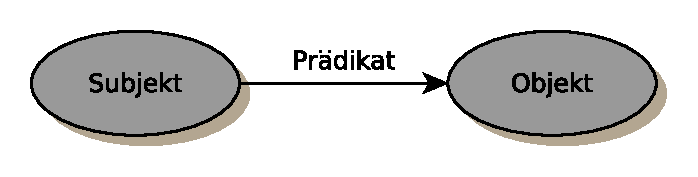
\includegraphics[
            width=0.6\textwidth,
            keepaspectratio=true,
            clip=true]
            {assets/images/rdf-triple}
        \caption{Einfacher RDF-Graph}
        \label{fig:graphisch_rdf_triple}
    \end{figure}

% paragraph graphische_darstellung (end)

\paragraph{RDF/XML} % (fold)
\label{par:rdf_xml}

RDF/XML\cite[Abschnitt 3.2]{Manola2004} ist eine verbreitete Form RDF-Dokumente zu beschreiben. Die Basis bildet hierbei die Verwendung der Extensible Markup Language (XML). In Listing \ref{lst:rdf_xml_beispiel} ist ein Beispieldokument in RDF/XML zusehen. Das in Zeile 2 zu sehende \texttt{rdf:RDF} Element zeigt, dass sich innerhalb von ihm sich die RDF-Beschreibung des Dokuments befindet. In diesem ELement werden mit \texttt{xmlns:} einige Präfixe für Namensräume  definiert, um das Dokument übersichtlicher zu halten. Alle Präfixe werden danach mit den angegebenen Namensraum ersetzt. Das \texttt{Description} in Zeile 5 stellt die Beschreibung einer Ressource im RDF-Graphen. Die URI der Ressource wird mit dem Attribut \texttt{rdf:about} definiert. Innerhalb des Description Elements befinden sich die Prädikate. In Zeile 6 steht also, dass die Ressource die Eigenschaft \texttt{exterms:enthaelt} besitzt und diese das Literal \texttt{Kekse}. Wäre das Objekt nicht wie hier ein Literal sondern eine weitere Ressource, könnte man über das Attribut \texttt{rdf:ressource} für das \texttt{exterms:enthaelt} auf diese Ressource verweisen.

\begin{lstlisting}[
    language=XML,
    caption={RDF/XML Beispiel}\label{lst:rdf_xml_beispiel},
    captionpos=t]
<?xml version="1.0"?>
<rdf:RDF xmlns:rdf="http://www.w3.org/1999/02/22-rdf-syntax-ns#"
    xmlns:exterms="http://www.example.org/terms#">

    <rdf:Description rdf:about="http://www.example.org/dose">
       <exterms:enthaelt>Kekse</exterms:enthaelt>
    </rdf:Description>
</rdf:RDF>
\end{lstlisting}
% paragraph rdf_xml (end)

\paragraph{Turtle} % (fold)
\label{par:turtle}

Turtle (Ausgeschrieben: \emph{Terse RDF Triple Language}) ist eine weiter Möglichkeit RDF-Graphen darzustellen und ist eine ging aus der Sprache N3 (Kurzform für Notation 2) hervor \cite{DavidBeckett}. In Turtle wird das Triple aus Subjekt, Prädikat und Objekt hintereinander geschrieben und zwischen jeden mindestens ein Leerzeichen gelassen. Als Abschluss folgt nach jedem Tripel noch ein Punkt. Der Punkt verdeutlicht noch einmal die Ähnlichkeit mit gesprochenen Sätzen. Listing \ref{lst:turtle_beispiel} zeigt das Beispiel mit der Keksdose noch einmal in Turtle Notation. 

\begin{lstlisting}[
    caption={Turtle Beispiel}\label{lst:turtle_beispiel},
    captionpos=t]
<http://www.example.org/dose> <http://www.example.org/terms#enthaelt> "Kekse" .
\end{lstlisting} 

In Turtle ist darauf zu achten, dass alle URIs immer zwischen Spitzenklammern stehen müssen. Literale werden in Anführungszeichen geschrieben. Da nun einzelne Prädikate beziehungsweise allgemein URIs recht häufig innerhalb eines Graphen auftauchen können, kann es einfacher sein diese abzukürzen. Wie schon in RDF/XML können auch in Turtle Präfixe definiert werden um Schreibarbeit zu sparen.

\begin{lstlisting}[
    caption={Turtle Präfixe}\label{lst:turtle_prefix},
    captionpos=t]
@prefix exterms: <http://www.example.org/terms#> .
<http://www.example.org/dose> exterms:enthaelt "Kekse" .   
\end{lstlisting}

In der ersten Zeile von Listing \ref{lst:turtle_prefix} wird durch Einleiten mit dem Schlüsselwort \texttt{@prefix} ein neuer Präfix \texttt{exterms:} für den Namensraum \texttt{http://www.example.org/terms\#}. Dieser Präfix kann nun überall innerhalb des Dokumentes verwendet werden, wobei die Spitzenklammern dann weggelassen werden können.

\begin{lstlisting}[
    caption={Turtle abkürzende Schreibweise}\label{lst:turtle_shortcut},
    captionpos=t]
@prefix exterms: <http://www.example.org/terms#> .
<http://www.example.org/dose> exterms:farbe "blau";
    exterms:enthaelt "Kekse", "Geld" .   
\end{lstlisting}

Listing \ref{lst:turtle_shortcut} zeigt nochmal ein drittes Beispiel, wie redundante Angeben eingespart werden. Wie man in der zweiten Zeile sehen kann. wir deine Frage für die Dose angeben das Triple aber mit einen Semikolon abschlossen und nicht mit einen Punk. Durch das Semikolon ist es Möglich das Subjekt mehrfach wieder zu verwenden, wenn sich nur Prädikat und Objekt ändern. So können sich mehrere Eigenschaften einer Ressource platzsparend schreiben ohne das Subjekt immer wieder anzugeben. Ändert sich dahingegen nur das Objekt können mehrere durch Kommata getrennt hintereinander geschrieben werden. Die dritte Zeile beschreibt zum Beispiel, dass in der Dose nicht nur Kekse sonder auch Geld steckt. Leere Knoten können dann noch in Turtle durch angeben einer geöffneten eckigen Klammer gefolgt von einer sich Schließenden dargestellt. Ein Beispiel für einen solchen leeren Knoten in Turtle ist in Listing \ref{lst:acl_beispiel} zu sehen.

% paragraph turtle (end)

% subsubsection darstellung_von_rdf (end)

\subsubsection{Ontologien} % (fold)
\label{ssub:ontologien}

% subsubsection ontologien (end)

% subsection semantic_web_und_das_resource_description_framework (end)

\subsection{Friend of a Friend (FOAF)} % (fold)
\label{sub:friend_of_a_friend_}

% subsection friend_of_a_friend_ (end)

\subsection{Semantically-Interlinked Online Communities (SIOC)} % (fold)
\label{sub:semantically_interlinked_online_communities}


Semantically-Interlinked Online Communities\footnote{\url{http://sioc-project.org/}} (SIOC, ausgesprochen \enquote{schock}) ist ein Projekt, welches von Uldis Boj\=ars und John Breslin begonnen wurde um unterschiedliche, webbasierte Diskussionslattformen(Blog, Forum, Mailinglist,\dots) untereinander verbinden zu können \cite{Breslin2005}. Der Kern von SIOC besteht aus einer Ontologie, welche den Inhalt und die Struktur diese Plattformen in ein maschinenlesbares Format bringt und es erlaubt diese auf semantischer Ebene zu verbinden. Auch soll es so möglich sein Daten von einer Plattform zu einer Anderen zu transferieren und so einfacher Inhalte austauschen zu können. Als Basis für SIOC dient RDF, die Ontologie selber wurde in RDFS und OWL designt. Um nicht das Rad neu erfinden zu müssen greift SIOC auf schon bestehende und bewährte Ontologien zurück. Für die Abbildung von Beziehungen zwischen einzelnen Personen wird Friend of a Friend\footnote{\url{http://www.foaf-project.org/}} (FOAF) und für einige Inhaltliche- und Metadaten (Titel, Inhalt, Erstelldatum, \dots) Dublin Core Terms\footnote{http://dublincore.org/documents/dcmi-terms/} eingesetzt.

\begin{figure}[ht]
    \centering
    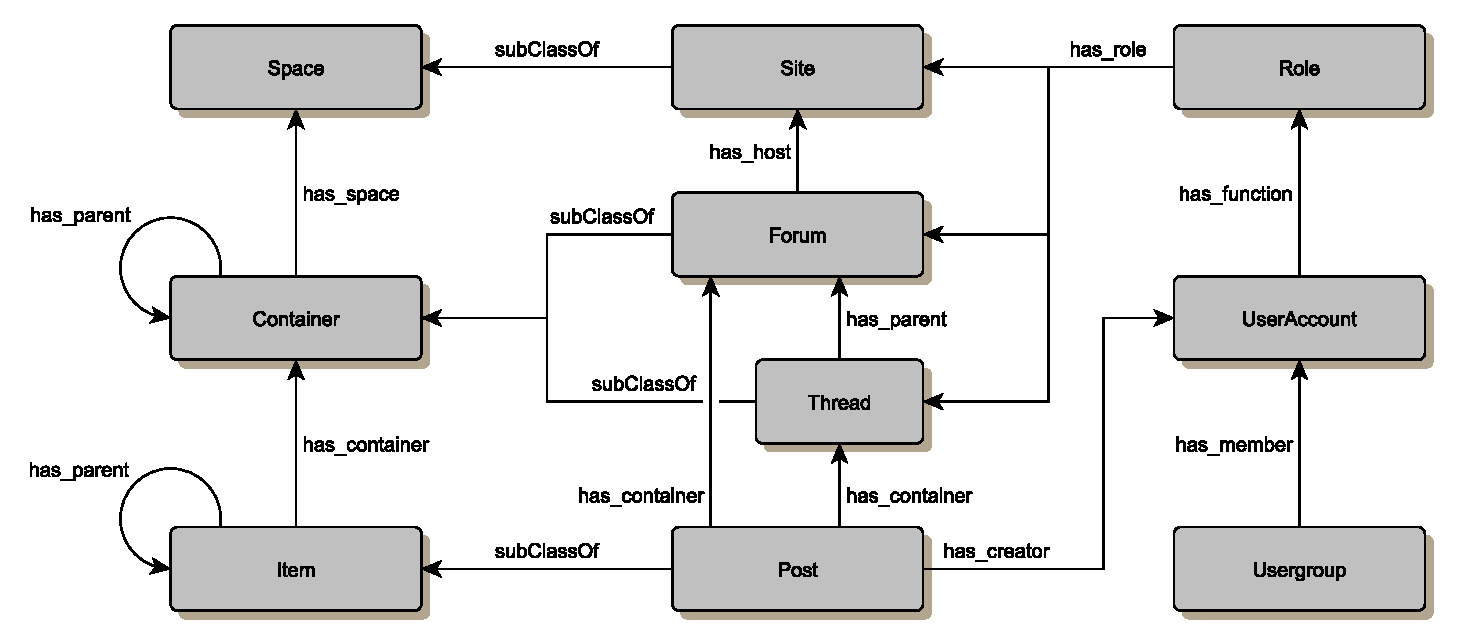
\includegraphics[
        width=\textwidth,
        keepaspectratio=true,
        clip=true]
        {assets/images/sioc_overview}
    \caption{Aufbau von SIOC (modifiziert) - Originalquelle: \cite{deri2013}}
    \label{fig:sioc_aufbau_diagramm}
\end{figure}

% subsection semantically_interlinked_online_communities (end)


\section{Datenverteilung} % (fold)
\label{sec:datenverteilung}

\subsection{Java Messaging Service} % (fold)
\label{sub:java_messaging_service}

% subsection java_messaging_service (end)

\subsection{Enterprise Integration Pattern und Apache Camel} % (fold)
\label{sub:enterprise_integration_pattern_und_apache_camel}

% subsection enterprise_integration_pattern_und_apache_camel (end)

% section datenverteilung (end)


\section{Lernplattformen und soziale Online-Netzwerke} % (fold)
\label{sec:lernplattformen_und_soziale_online_netzwerke}

An dieser Stelle sollen noch kurz einige Lernplattformen und soziale Online-Netzwerke vorgestellt, die im späteren Verlauf dieser Arbeit für die Implementierung verwendet wurden. Im Einzelnen waren dies \emph{Moodle}, \emph{Canvas}, \emph{Youtube}, \emph{Facebook} und \emph{Google+}, da sie einen guten Schnitt von den Plattformen bilden, die heutzutage sowohl im Bereich E-Learning als auch von der breiten Masse verwendet werden.

%\todo[inline]{Du könntest in dem Grundlagenkapitel auch noch auf Foren, Moodle, FB und Google+ kurz eingehen. Deren Datenmodelle und -schnittstellen können auch später erläutert werden.}

\subsection{Moodle} % (fold)
\label{sub:moodle}

Moodle\footnote{\url{https://moodle.org/}} ist ein weit verbreitetes Open Source Online LMS. Die Hauptaufgabe liegt im Verwalten von online Kursen im Bereich E-Learning. Hierzu bietet Moodle von Haus aus eine große Menge an Funktionen für die Verwaltung des Kurses und die Kommunikation zwischen Lehrenden und Lernenden. Es bietet die Möglichkeit Aufgaben die Teilnehmern zu verteilen, Fragebögen zu erstellen, zusätzlichen Kursmaterialien bereitzustellen und den Lernerfolg durch Benotung und Feedback zu kontrollieren. Funktionen für die Unterstützung des kooperativen Lernens sind ebenfalls vorhanden. Teilnehmer können Lerngruppen bilden, sich über persönliche Nachrichten austauschen, gemeinsam an Wikis arbeiten oder in Foren diskutieren. 
\begin{figure}[ht]
    \centering
    \includegraphics[
        width=0.7\textwidth,
        keepaspectratio=true,
    ]{assets/images/tud_moodle_screenshot}
    \caption{Moodle Instanz der TU Darmstadt}
    \label{fig:moodle_tud}
\end{figure}

\medskip

Moodle wurde in der Programmiersprache PHP geschrieben und unterstützt die  Datenbanken werden MySQL, PostgrSQL, MSSQL und Oracle. Die Installation von weiteren Funktionalitäten ist durch von Dritten geschriebenen Erweiterungen möglich. Seit Version 2.0 können für Moodle auch Webservices installiert werden, so können auch externe Anwendungen auf interne Funktionen und Daten zugreifen.

% subsection moodle (end)

\subsection{Canvas} % (fold)
\label{sub:canvas}

Das von der Firma Instructure\footnote{\url{https://www.instructure.com/}} entwickelte \emph{Canvas} ist ein unter Open Source Lizenz gestelltes LMS. Vom Funktionsumfang ist es Moodle nicht unähnlich. Es existiert eine Verwaltung einzelner Kurse. Innerhalb dieser Kurse können in einem Forum Diskussionen geführt und Lernmieteralien hoch- und heruntergeladenen werden. Verteilung von Aufgaben, deren Benotung und ein Benachrichtigungssystem existiert ebenfalls. Canvas erlaubt auch das Einbinden von externen Diensten zum kooperativen Lernen und Arbeiten wie Google Docs\footnote{\url{https://drive.google.com}} oder der Webkonferenz Anwendung BigBlueButton\footnote{\url{http://www.bigbluebutton.org}}.

\begin{figure}[ht]
    \centering
    \includegraphics[
        width=0.7\textwidth,
        keepaspectratio=true,
    ]{assets/images/canvas_lms}
    \caption{Instructure Canvas}
    \label{fig:canvas_lms}
\end{figure}

Canvas wird mittels des Webframeworks \emph{Ruby on Rails}\footnote{http://rubyonrails.org/} entwickelt. Das Aussehen ist etwas moderner, als das von Moodle und es wird sehr stark auf die neuesten Webtechnologien wie HTML5 CSS3 und JQuery gesetzt. Eine Erweiterung der Funktionalität von Canvas ist durch das einbinden von Programmen möglich, die den \emph{Learning Tools Interoperability™} (LTI) Standard erfüllen. Einige solcher Programme finden sich auf der Webseite \url{https://www.edu-apps.org}. Unter anderem Programme zum Suchen und Einbinden von Youtube Videos, Wikipedia Artikeln, GitHub Gists\footnote{\url{https://gist.github.com}} und vielen weiteren.

% subsection canvas (end)

\subsection{Youtube} % (fold)
\label{sub:youtube}

Die Youtube\footnote{\url{https://www.youtube.com}} Webseite gehört wohl heute zu den beliebtesten Anlaufpunkten im Internet, wenn es um das Thema Videos geht. Monatlich nutzen über 1 Milliarde Nutzer die Seite und pro Minute werden 100 Stunden neuer Videos hochgeladen \cite{youtube2013statistics}. Doch nicht das komplette Videomaterial besteht aus Katzen, Musik oder Videos von Unfällen. Ein Teil der Benutzer die eigene Videos hochladen, wollen anderen Dinge beibringen, weil es sie schon immer interessierte oder früher selber Probleme damit hatten. Einer erklärt die Logarithmengesetze, ein anderer wie man Feuer ohne Feuerzeug macht und eine ganz andere gibt Schönheitstipps. Youtube ist also auch im E-Learning Bereich gut einsetzbar. Lehrende können eigene Videos hochladen, von anderen interessante Videos in Playlisten zusammenfassen und die Lernenden können über Kommentare Fragen zum Inhalt stellen. 

% subsection youtube (end)

\subsection{Facebook} % (fold)
\label{sub:facebook}

Das soziale Online-Netzwerk Facebook\footnote{\url{https://www.facebook.com/}} kann mit rund 699 Millionen aktiven Benutzern täglich \cite{Facebook2013} zu den aktuell beliebtesten Vertretern seiner Art bezeichnet werden. Facebook erlaubt es, wie alle sozialen Online-Netzwerke, bekannte Personen in Freundeslisten zusammen zufassen und mit ihnen private Nachrichten auszutauschen. Beiträge wie Texte, Fotos oder Videos können auf einer Art Pinnwand der \enquote{Wall} öffentlich oder nur mit Freunden geteilt werden. Benutzer mit gemeinsamen Interessen können dazu eigene Gruppen bilden und dort auf einer eigen Wall Beiträge veröffentlichen oder die anderer kommentieren. Wie in der Einleitung schon erklärt zeigt Qiyun Wang et. al. \cite{Wang2012} das sich Facebook, wenn auch mit Einschränkungen wunderbar zur Verwaltung und Nutzung durch Lernkurse und Lerngruppen eignet. 


% subsection facebook (end)

\subsection{Google+} % (fold)
\label{sub:google_plus}

Google+\footnote{https://plus.google.com} ist ein 2011 von Google gestartetes soziales Online-Netzwerk. Seit Anfang 2013 ist Google+, von der Anzahl der aktiven Benutzer her gesehen, auf Platz 2 hinter Marktführer Facebook \cite{Thomas2013}. Vom Funktionsumfang sind sich beide sehr ähnlich. Auf Google+ können andere Benutzer in sogenannten \enquote{Circles} sortiert werden. Dies entspricht ungefähr den auf Facebook genutzten Freundeslisten. Jeder Benutzer hat einen eigenen \enquote{Stream} in dem er Beiträge öffentlich oder nur für ein oder mehrere Circles verfassen kann. Das Gründen von Gruppen für bestimmte Interessensbereiche ist auch in Google+ möglich und werden dort als \enquote{Communities} bezeichnet. Eines der interessantesten Funktionen von Google+ dürfte die Einführung von \enquote{Google Hangout} sein. Hier können Benutzer neben Chats auch Videokonferenzen mit bis zu zehn anderen abhalten, ohne einen externen Service wie Skype\footnote{\url{http://www.skype.com/}} zu nutzen. Diese Funktion wäre gut für den Einsatz in E-Learning nutzbar. Ein Tutor könnte so in kleiner Runde Fragestunden abhalten oder Gruppen Treffen abhalten.

% subsection google_ (end)

% section lernplattformen_und_soziale_online_netzwerke (end)

\section{Verwandte Arbeiten und Projekte} % (fold)
\label{sec:verwandte_arbeiten_und_projekte}


\subsection{What happens when Facebook is gone?} % (fold)
\label{sub:what_happens_when_facebook_is_gone}

Frank McCown und Michael L. Nelson beschreiben in ihrem Bericht \enquote{What happens when Facebook is gone?}\cite{McCown2009}, wie Möglichkeiten aussehen können, die unsere Daten von sozialen Online-Netzwerken (hier im speziellen Fall von Facebook) für uns und die Nachwelt archivieren können. Zum Beispiel, wenn eine Person einen großen Teil seines persönlichen Lebens auf Facebook verbringt und plötzlich stirbt. Wie sollen seine Angehörigen an nicht öffentliche Texte, Bilder, Videos heran kommen, wenn sie in der Regel keinen Zugriff auf das Benutzerkonto haben, da der Verstorbene so etwas nicht vorhersehen konnte. Oder wenn ein Benutzer mit seinen Daten in ein anderes soziales Online-Netzwerk umziehen will, sei dies bei Facebook zum damaligen Zeitpunkt nur schwer möglich.

\begin{quote}
    \enquote{It is also likely he was not prepared to die at such a young age, and much of his personal life, which lies in the digital \grqq cloud\grqq, may never be accessible to his loved ones}
    \cite[S.\,251]{McCown2009}
\end{quote}

Zum Anlegen eines solchen Archivs wurden mehrere Ansätze vorgestellt. Die einfachste Ansatz wäre die E-Mail-Benachrichtigung zu aktivieren und alle neuen Beiträge in einem E-Mail-Postfach zu sichern. So können aber nur neuen alle Beiträge erfasst werden, alte bleiben weiterhin in Facebook. Eine sehr aufwändige Möglichkeit wäre es Bildschirmfotos von den Beiträgen zu machen und diese durch ein Texterkennungsprogramm laufen zu lassen. Die dadurch erzeugten Dateien können dann in einer Datenbank gespeichert werden. Heutige Internetbrowser zusätzlich zum Anzeigen von Webseite auch der Herunterladen selbiger an. Dabei wird die HTML-Datei inklusive aller darin enthaltenen weiteren Dateien wie Bilder, Videos und CSS-Dateien gespeichert. Die so archivierte Seite hat dann im beschränkten Umfang genau das gleiche Aussehen und Verhalten wie die original Seite. Ebenfalls wäre eine Nutzung der von Facebook bereitgestellten API für Anwendungen eine Überlegung wert. 2009 war diese API noch sehr eingeschränkt. Gerade der Zugriff auf Beiträge und private Nachrichten war nicht möglich \cite[S.\,253, Table 1]{McCown2009}. Für die Implementierung eines Beispiel Programms wurde ein fünfter Ansatz gewählt. Über einen sogenannten Webcrawler oder eine Erweiterung für den Browser werden relevante Seiten automatisch heruntergeladen und in einen Archiv abgelegt. Dynamische Inhalte sollen kein Problem darstellen, da Seite erst heruntergeladen wird, wenn alle Aufrufe dynamischer Funktionen abgeschlossen ist. Die archivierten Dateien können dann mittels Datamining Techniken verarbeitet und als Atom/RSS Feed\footnote{\url{http://www.rssboard.org/rss-specification}} bereitgestellt werden. 

% subsection what_happens_when_facebook_is_gone_ (end)

\subsection{Reclaim Social} % (fold)
\label{sub:reclaim_social}

Hat sich nicht jeder schon einmal vor den Rechner gesessen um, zum Beispiel, nach einen Bild gesucht das man irgendwann auf irgendeinem der unzähligen sozialen Netzwerke hochgeladen hat, einem aber partout nicht einfallen will wo? Wann und wo habe habe ich den Beitrag geschrieben, der perfekt zu meiner aktuellen Arbeit passen würde? Solche oder ähnliche Fragen wurden sicherlich schon mehrere Millionen mal von verschiedenen Menschen in der Welt des Internets gestellt. Wer hätte in so einen Fall nicht gerne alles was man über die letzten Jahre an verschiedenen Stellen im Netz geschrieben, hochgeladen oder als für ihn wichtig markiert hat zentral gespeichert um es durchsuchen zu können? Genau diesem Thema haben sich Sascha Lobo und Felix Schwenzel angenommen und auf der Netzkonferenz re:publica\footnote{\url{http://re-publica.de/}} 2013 ihr gestartetes Projekt \enquote{Reclaim Social} \cite{Schwenzel2013} vorgestellt.

\todo[inline]{Das klingt ein wenig wie ein Werbetext ;-)}

\medskip

Ziel mit diesem Projektes soziale Medien aus allen möglichen Quellen auf seinen eigenen Blog zu spiegeln und so einen zentrale Anlaufstelle für seine eigenen Inhalte schaffen. Aufbauend auf der weit verbreiteten Blogsoftware \enquote{WordPress\footnote{\url{http://wordpress.org/}}} und der dafür vorhandenen Erweiterung \enquote{FeedWordPress}\footnote{\url{http://feedwordpress.radgeek.com/}}. Diese Kombination ermöglichst alle Internetseiten, welche einen RSS Feed anbieten, in die Datenbank von WordPress zu spiegeln. Das Problem hierbei besteht darin, dass einige sehr beliebte Internetseiten solche RSS Feeds nicht anbieten (Facebook, Google+) oder eingestellt haben (\url{https://twitter.com}). Für einige solcher Seiten wurden \enquote{proxy-scripte}\cite[Tech Specs Details]{Schwenzel2013} implementiert, welche für diese einen RSS Feed emulieren. Zugleich können in den Feeds enthaltende Medien, wie Bilder und Videos(bisher nur als Referenz), heruntergeladen und in WordPress gespeichert werden. So ist es möglich alle gespiegelten Daten einfach zu durchsuchen oder nach bestimmten Kriterien zu filtern. Zusätzlich können alle Freunde, welche auch Reclaim Social einsetzen, in einen Kontaktliste eingetragen und so auch deren Inhalte eingebunden werden.

\medskip

Aktuell befindet sich dieses Projekt noch im Alpha Stadium und die Installation ist relativ kompliziert. Es ist aber geplant eine eigene Erweiterung für WordPress zu schreiben \enquote{he goal is to build just one Reclaim Social-plugin for any wordpress user}\cite[How Does It Work]{Schwenzel2013}

% subsection reclaim_social (end)

% section verwandte_arbeiten_und_projekte (end)

% chapter grundlagen (end)
		%!TEX root = ../thesis.tex

\chapter{Analyse} % (fold)
\label{cha:analyse}

%\todo[inline]{Inhalt: wass gibt es, was muss neu gemacht werden}
\todo[inline]{Aufteilen in Szenarien: Datenaustausch, Übertragung...}

Bevor nun ein System entwickelt werden kann, das die Synchronisation von Diskussionen auf Lernplattformen und sozialen Online-Netzwerken ermöglicht, muss erst analysiert werden, welche Aufgaben das System erfüllen muss und welche Techniken dafür geeignet sind. Alle diese Schritte sollen im folgenden Abschnitt an einen kleinen Beispiel gezeigt werden.

\section{Ein Beispiel} % (fold)
\label{sec:analyse_beispiel}

% section neuen_beitrag_verfassen (end)
Am Anfang muss irgendjemand auf einer Webseite einen Beitrag schreiben der synchronisiert werden kann. Zum Beispiel geht ein Student in das Forum seiner Veranstaltung auf der Webseite A und in den Thread zur aktuellen Übung, weil er zu ihr eine Frage hat. Er schreibt also einen neuen Beitrag in das Eingabefeld und schickt es ab. Dieser wird dann an die Webseite A geschickt, im dortigen Format (Format A) in eine Datenbank oder Ähnliches geschrieben und als neuer Beitrag im Thread angezeigt (siehe Abbildung \ref{fig:beutzer_erstellt_beitrag_a}). Da eine andere Webseite B das Format von Webseite A in der Regel nicht versteht, muss in einen nächsten Schritt der Beitrag aus der Datenbank gelesen und auf irgendeine Art konvertiert werden. 

\begin{figure}[ht]
     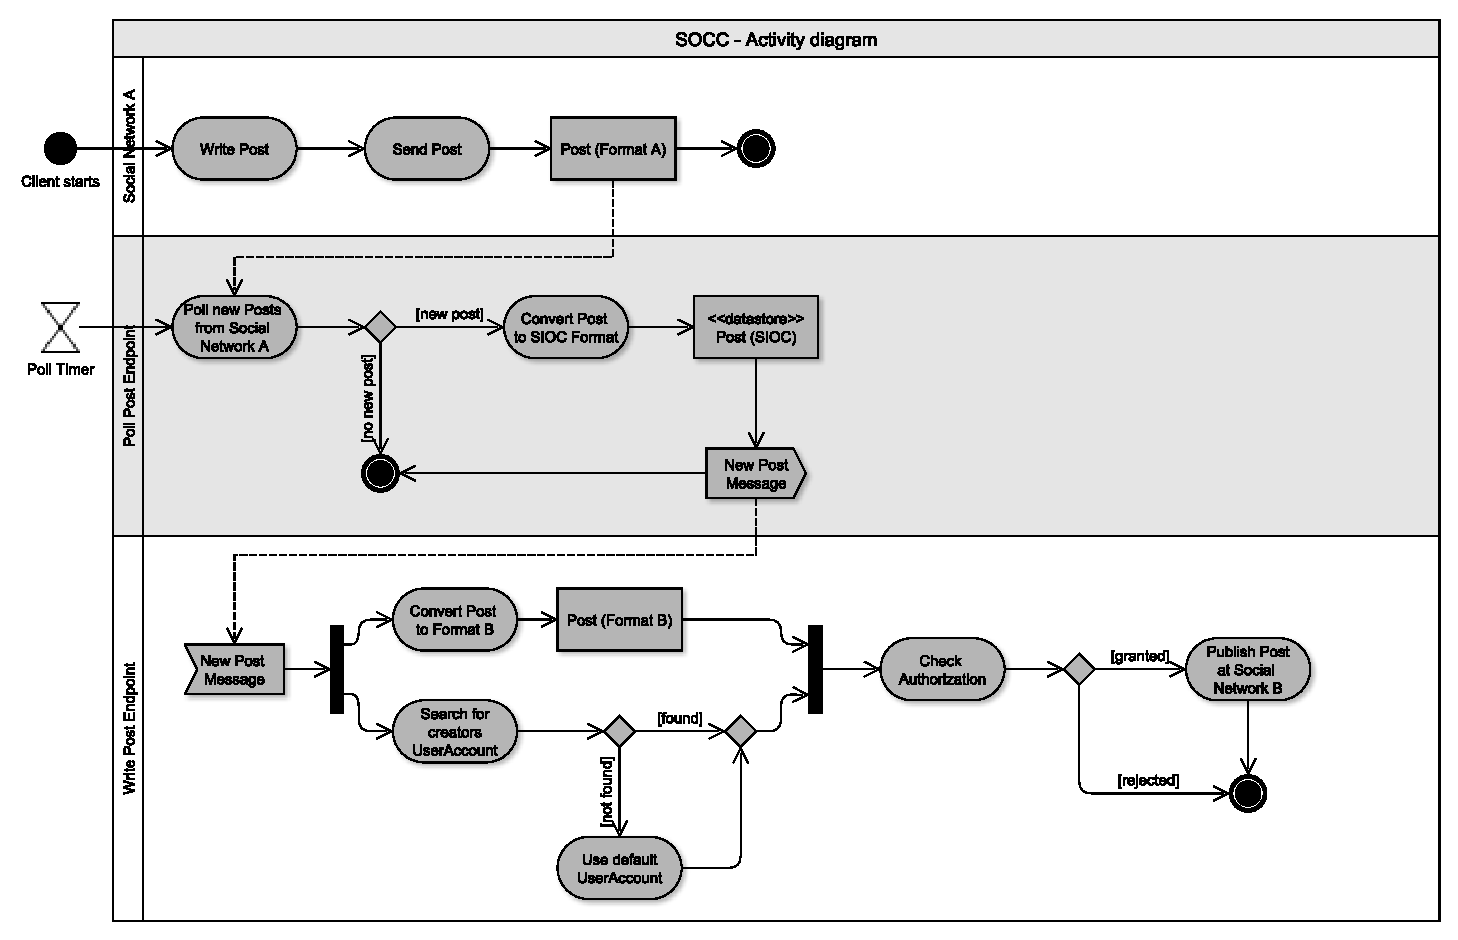
\includegraphics[
        width=\textwidth,
        keepaspectratio=true,
        clip=true,
        trim= 0 338 0 27
    ]{assets/images/activitydiagram_post_as_user_check_authorization.pdf}
    \caption{Benutzer erstellt einen Beitrag im sozialen Netzwerk A.}
    \label{fig:beutzer_erstellt_beitrag_a}
\end{figure}

\subsection{Beiträge lesen und konvertieren} % (fold)
\label{sub:beiträge_lesen_und_konvertieren}

Abbildung \ref{fig:lesen_von_beitrag_und_convertieren} zeigt den Ablauf, wie Beiträge von der Webseite A gelesen, konvertiert und weiterverarbeitet werden. Dazu müssen zuerst die Daten über eine öffentliche API vom Server des Webseite A heruntergeladen werden. Da im Allgemeinen nicht automatisch bekannt ist, wann ein neuer Beitrag vorhanden ist, müssen die Server in zeitlichen Abständen abgefragt (\emph{Polling} genannt) und die zurückgelieferten Daten nach neuen Beiträgen durchsucht werden. Sind ein oder mehrere neue Beiträge gefunden worden, können diese nicht direkt an die Webseite B geschickt werden, da sich diese in der Regel im verwendeten Datenformat unterscheiden. Diese müssen zuvor konvertiert werden.

Die einfachste Möglichkeit wäre die Daten von Webseite A, die in Format A vorliegen, in das Format B von Webseite B zu konvertieren. Bei zwei Formaten ist dies noch sehr einfach. Es müsste lediglich ein Konverter von Format A nach Format B und einer in die umgekehrte Richtung implementiert werden. Für den Fall, dass ein weiteres Webseite C unterstützt werden soll, würde ich die Anzahl an notwendigen Konvertern , wie Tabelle \ref{tbl:anzahl_konvertern_bei_drei_netzwerken} zeigt, auf Sechs erhöhen.

\begin{table}[ht]
    \centering
    \caption{Anzahl Konverter bei drei Webseiten}
    
    \begin{tabular}{c|c|c|c|c}
        % Zeile 1
        \multicolumn{2}{c|}{\multirow{2}{*}{}} & 
        \multicolumn{3}{|c}{\textbf{Nach}}   \\ 
        \cline{3-5} 

        % Zeile 2
        \multicolumn{2}{c|}{} & 
        \textbf{Webseite A} & 
        \textbf{Webseite B} & 
        \textbf{Webseite C} \\ 
        \hline

        % Zeile 3
        \multirow{3}{*}{Von} & 
        \textbf{Webseite A} & 
        -&            
        $ \times $ &            
        $ \times $ \\ 
        \cline{2-5} 

        % Zeile 4
        & 
        \textbf{Webseite B} &            
        $ \times $ &            
        -&            
        $ \times $ \\ 
        \cline{2-5} 
         
        % Zeile 5
        & 
        \textbf{Webseite C} &            
        $ \times $ &            
        $ \times $ &            
        -\\
    \end{tabular}
    \label{tbl:anzahl_konvertern_bei_drei_netzwerken}
\end{table}

Nimmt man an $n_{ws}$ sei eine beliebige Anzahl sozialer Netzwerke, entspricht die Anzahl der notwendiger Konverter $ n_{k1} = n_{ws}*(n_{ws}-1) $, da für jedes Netzwerk ein Konverter in alle anderen Netzwerke erzeugt werden muss. Sollen nur Zwei oder Drei Netzwerke unterstützt werden ist der Aufwand noch sehr überschaubar, bei mehr kann dies aber sehr Aufwendig werden. 

\begin{figure}[ht]
    \centering
    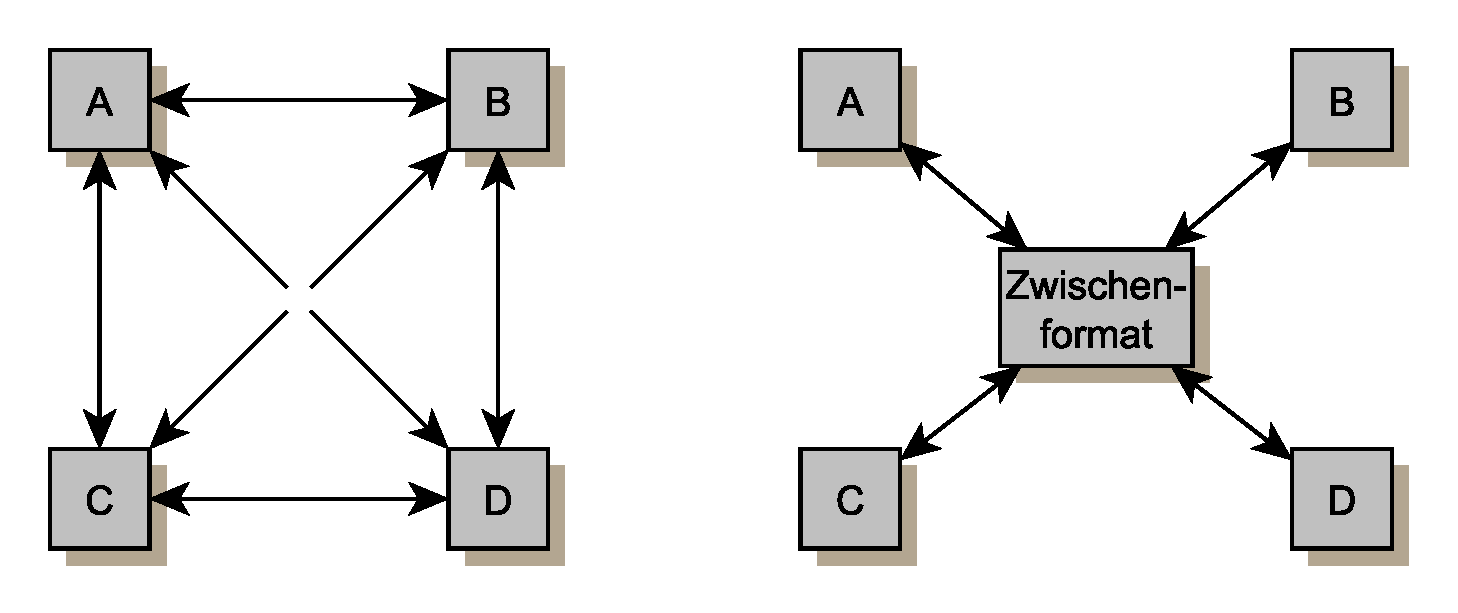
\includegraphics[
        width=0.7\textwidth,
        keepaspectratio=true
    ]{assets/images/interlingua_vs_allvsall}
    \caption{Komplexität ohne und mit dem Einsatz eines Zwischenformats - Originalbild: \cite{Uschold1996a}}
    \label{fig:interlingua_vs_all}
\end{figure}

Eine elegantere Methode für die Lösung dieses Problems, welche die Anzahl zu implementierender Konverter in Grenzen halten kann, wäre die Einführung eines Zwischenformates (auch Inter-Lingua, in Abbildung \ref{fig:lesen_von_beitrag_und_convertieren} als \enquote{IM Format} bezeichnet) \cite[S.\,9]{Uschold1996a}. Geht man davon aus, dass die Daten aller Webseiten nur in dieses Zwischenformat geschrieben und aus diesem gelesen werden müssen, würde sich der Aufwand auf maximal zwei Konverter je Webseite reduzieren. Für eine beliebige Anzahl Webseiten wären also $ n_{k2} = n_{ws} * 2 $ Konverter nötig. Nachteile hätte dieser Ansatz nur für $ n_{ws} = 2 $ und $ n_{ws}=3$ , da in diesen Fällen mehr beziehungsweise gleich viele Konverter gegenüber der ersten Methode erforderlich wären. Erhöht man die Anzahl Webseiten jedoch nur geringfügig, sinkt die Menge an Konvertern sichtbar. Für $ n_{ws} = 4 $ wären es $ n_{k2} = 8 $ statt $ n_{k1} = 12 $ (siehe Abbildung \ref{fig:interlingua_vs_all}) und für $ n_{ws} = 5 $ ergibt sich $ n_{k2} = 10 $ statt $ n_{k1} = 20 $ Konvertern. Gleichzeitig können so syntaktische Unterschiede in den einzelnen Formaten angeglichen werden, was sie leichter handhabbar macht. 

\begin{figure}[ht]
    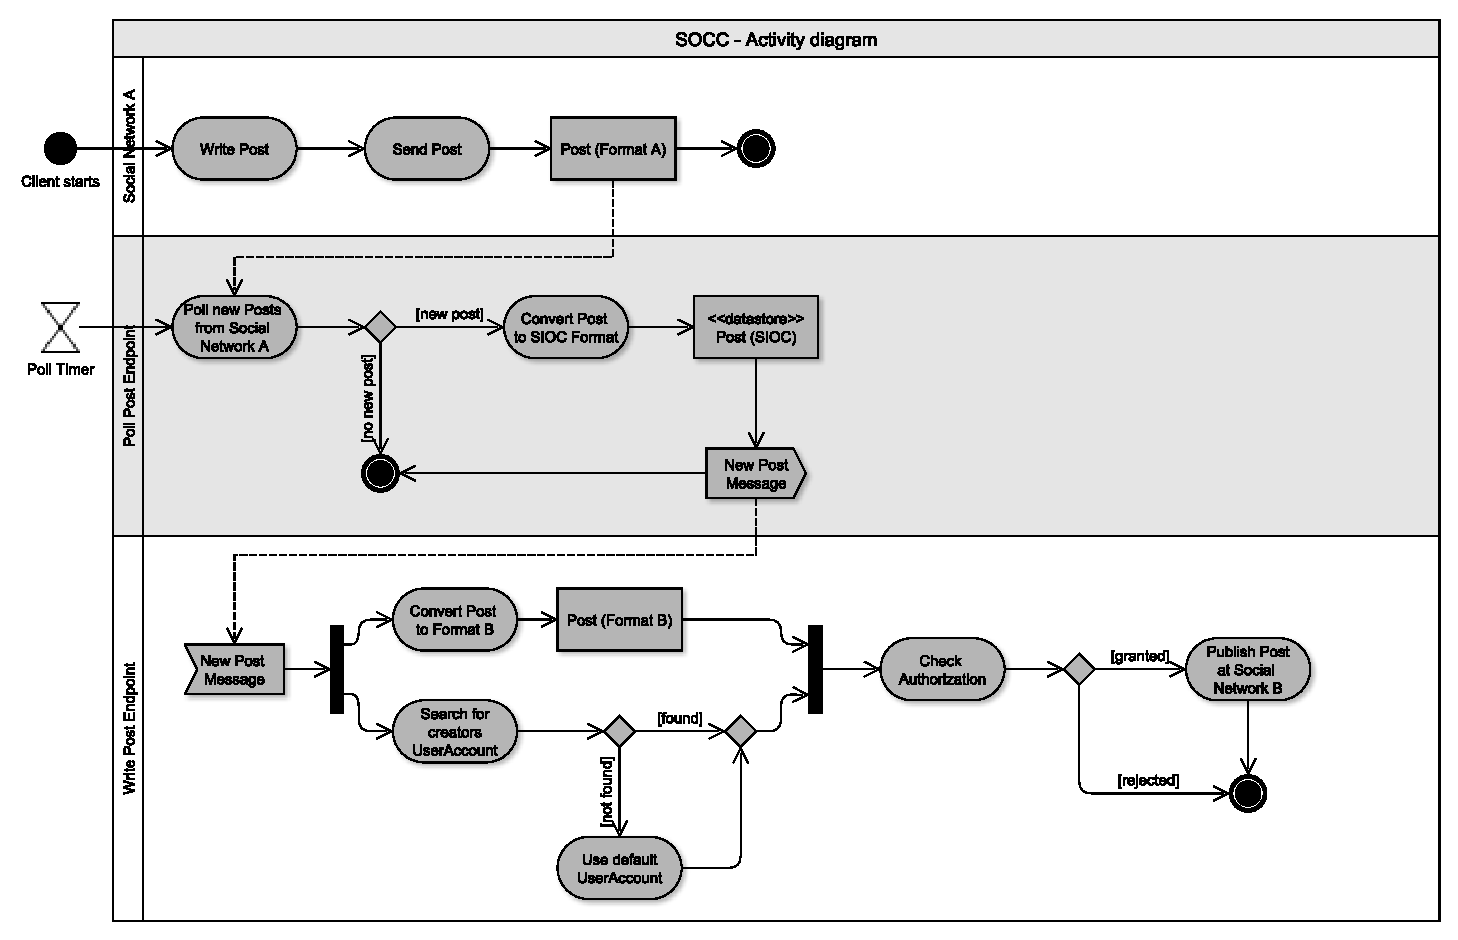
\includegraphics[
        width=\textwidth,
        keepaspectratio=true,
        clip=true,
        trim= 0 193 0 113
    ]{assets/images/activitydiagram_post_as_user_check_authorization.pdf}
    \caption{Lesen des erstellten Beitrags und konvertieren in das Zwischenformat.}
% section beiträge_von_solzialen_netzwerk_a_lesen (end)
    \label{fig:lesen_von_beitrag_und_convertieren}
\end{figure}

Bei der automatischen Sammlung von benutzergenerierten Inhalten stellt sich immer die Frage der Privatsphäre. Nicht jeder möchte, dass vielleicht sensible Informationen von ihnen weitergegeben werden. Aus diesem Grund ist die Einführung eines Mechanismus sinnvoll mit dem ein Benutzer das Lesen seiner Beiträge komplett erlaubt oder auf bestimmte Seiten, Foren oder nur für einzelne Threads beschränkt \cite{Bojars2011}. Sollte eine solche Erlaubnis nicht vorliegen, wird der gelesene Beitrag verworfen.

Da das Eintreffen neuer Beitrage nicht vorhersagbar ist, ist es angebracht beim Synchronisieren das Lesen und Schreiben zeitlich zu entkoppeln. Eine der weit verbreitetsten Techniken dazu ist das Versenden von Nachrichten über einen Nachrichtenkanal den die schreibende Komponente nach neuen Beiträgen abhört. Diesen Kanal können mehrere Gleichzeitig abhören und stellen so eine gute Flexibilität sicher. 

% subsection beiträge_lesen_und_konvertieren (end)

\subsection{Beiträge in eine andere Webseite schreiben} % (fold)
\label{sub:beiträge_in_eine_andere_webseite_schreiben}


Empfängt nun eine Komponente, die für das Schreiben zuständig ist, eine Nachricht von einen neuen Beitrags der Webseite A ist der Ablauf ähnlich wie beim Lesen nur in umgekehrter Reihenfolge (Siehe Abbildung \ref{fig:konvertieren_formatb_und_schreiben} links, oberer Ablauf). Der neue Beitrag wird vor dem Schreiben aus dem Zwischenformat in das Format B konvertiert. Da bei einer Synchronisation vom Vorteil wäre, wenn der synchronisierte Beitrag so aussehen würde, als hätte ihn der original Autor geschrieben. Hierzu muss das System Zugriff auf die Benutzerkonto haben und diese in einer Datenbank verwalten. Dort kann dann nach einen passenden Benutzerkonto des Autors gesucht und dieses dann zum Schreiben verwendet werden. Steht ein solches Benutzerkonto nicht zur Verfügung, ist das Ausweichen auf ein vorgegebenes Benutzerkonto hilfreich. Manche Benutzer sind vielleicht damit einverstanden, dass ihre Beiträge weitergegeben werden, aber nicht dass andere Programme automatisch in ihren Namen Beiträge schreiben. Deswegen ist wichtig davor noch einmal zu prüfen, ob eine entsprechende Erlaubnis gegen wurde. Sind alle Voraussetzungen gegeben, kann der Beitrag über das ausgewählte Benutzerkonto auf die Webseite B geschrieben werden.

\begin{figure}[ht]
     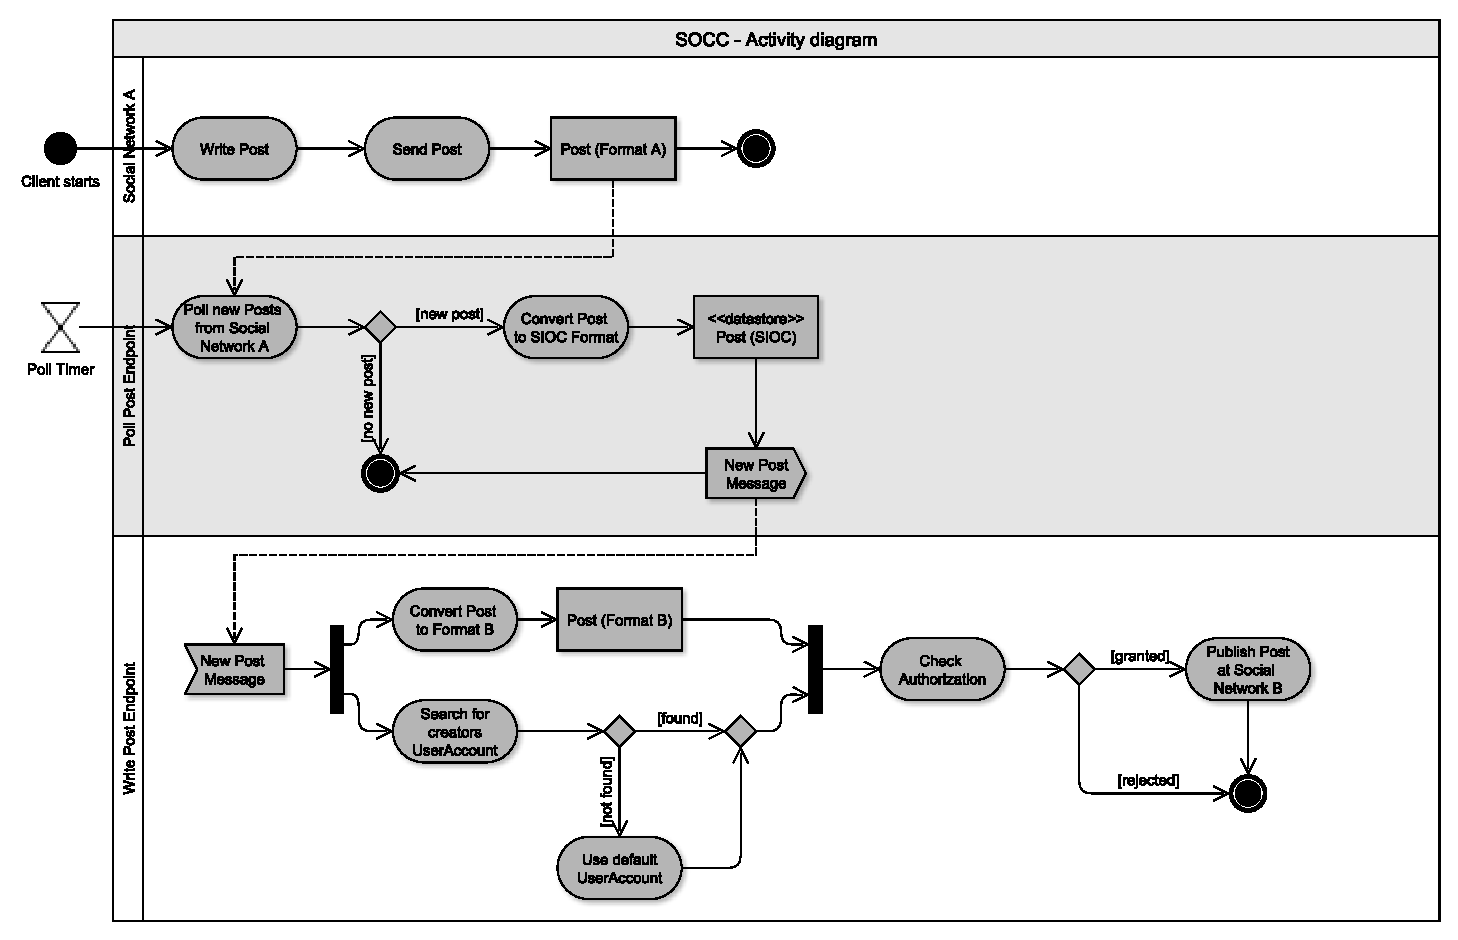
\includegraphics[
        width=\textwidth,
        keepaspectratio=true,
        clip=true,
        trim= 0 0 0 257
    ]{assets/images/activitydiagram_post_as_user_check_authorization.pdf}
    \caption{Konvertierten des Beitrags in das Format B und schreiben n das soziale Netzwerk B}
    \label{fig:konvertieren_formatb_und_schreiben}
\end{figure}

% subsection beiträge_in_eine_andere_webseite_schreiben (end)

\section{Identifizierung der Komponenten} % (fold)
\label{sec:identifizierung_der_komponenten}

Anhand dieses kurzen Ablaufbeispiels kann man einige Komponenten ablesen, aus denen das neue System auf jeden Fall bestehen beziehungsweise enthalten muss und welche ergänzend dazu Wünschenswert wären:

\begin{itemize} 
    \item Eine Komponente muss Daten von einen Webseite über deren öffentlicher API in das System einlesen und diese in ein geeignetes Zwischenformat konvertieren können.
    \item Es muss ein passendes Nachrichtensystem zum Entkoppeln von Lesen und Schreiben gewählt und/oder erstellt werden.
    \item Eine weitere Komponente nimmt Beiträte im Zwischenformat entgegen, konvertiert diese in das Format des entsprechenden Netzwerkes und schreibt diese dorthin.
    \item Um stellvertretend für einen Benutzer schreiben zu können, muss es möglich sein nach dem Konto eines Benutzer zu einer bestimmten Webseite suchen zu können.
    \item Um die Privatsphäre der Benutzer zu wahren, wäre eine Mechanismus zum festlegen von Zugriffsrechen sinnvoll.
\end{itemize}   

% section identifizierung_der_komponenten (end)

\section{Wahl vorhandener Techniken} % (fold)
\label{sec:wahl_vorhandener_techniken}

\todo[inline]{vielleicht doch eher an den Anfang von "Eigener Ansatz"!?}

\subsection{Welches Zwischenformat?} % (fold)
\label{sub:welches_zwischenformat}

Ein passendes Zwischenformat wurde im Kapitel \enquote{\ref{cha:grundlagen}} mit SIOC beziehungsweise die Kombination aus SIOC und FOAF bereits vorgestellt. Damit ist es nicht nur möglich einzelne Beiträge plattformunabhängig zu speichern, sondern es kann auch die Struktur der Plattform als auch der Benutzer mit eingebunden werden. Auch können Maschinen aus den RDF-Daten einfach Wissen für neue, hilfreiche Informationen ableiten. Doch warum sollte man auf RDF und Ontologien setzen anstatt etwas eigenes zu Entwickeln wie auf Basis des weitverbreiteten und vielseitigen XML Formats?

Hier gibt es mehrere Vorteile, warum man RDF einer mit XML-Schema definierten XML-Datei vorziehen sollte. XML hat das Problem, dass die selbe Aussage auf verschiedene Art repräsentiert werden kann. Listing \ref{lst:xml_vs_rdf_multiple_rep} zeigt ein Beispiel für die Repräsentation der Aussage \enquote{Max Hiwi ist der Autor des Beitrags mit der ID 42} in XML.

\begin{lstlisting}[
    language=XML,
    caption={XML: Unterschiedliche Syntax, gleiche Semantik }\label{lst:xml_vs_rdf_multiple_rep},
    captionpos=t]
    <post>
        <id>42</id>
        <author>Max Hiwi</author>
    </post>

    <post id="42">
        <author>Max Hiwi</author>
    </post>

    <post id="42" author="Max Hiwi" />
\end{lstlisting}

Alle drei XML-Elemente beschreiben die selbe Aussage, aber auf unterschiedliche Art und Weise. Für einen Menschen haben diese drei Schreibweisen die selbe Aussage, für eine Maschine ist dies aber nicht mehr ganz so offensichtlich. Auch kann nicht die Bedeutung der einzelnen Element und Tags von Maschinen erfasst werde. Dies muss der Programmierer erledigen.Zusätzlich erschweren diese Unterschiedlichen Strukturen das ausführen von Abfragen auf diesen Daten, da ein Mapping zwischen einer logischen Abfrage und den Daten nicht eindeutig erfolgen kann (vgl. \cite[s.\,41]{Schroder2003a}).

% subsection welches_zwischenformat (end)

\subsection{Welches Nachrichtensystem?} % (fold)
\label{sub:welches_nachrichtensystem}

\subsubsection{JMS} % (fold)
\label{ssub:analyse_jms}
\begin{itemize}
    \item zum reinen verschicken ausreichend
    \item fast alles muss selber gemacht werden.
\end{itemize}
    
\subsubsection{Apache Camel} % (fold)
\label{ssub:analyse_apache_camel}
    \begin{itemize}
        \item erweitern der "Pipeline" z.B. mit Filtern einfach möglich
    \end{itemize}

\subsubsection{JMS + Apache Camel} % (fold)
\label{ssub:analyse_jms_apache_camel}

\begin{itemize}
    \item gute kombination -> durable subscriber
\end{itemize}

% subsubsection analyse_jms_apache_camel (end)

% subsubsection analyse_apache_camel (end)

% subsubsection analyse_jms (end)

% subsection welches_nachrichtensystem (end)

% section wahl_vorhandener_techniken (end)

% chapter analyse (end)
		%!TEX root = ../thesis.tex

\chapter{Eigener Ansatz} % (fold)
\label{cha:eigener_ansatz}


\begin{itemize}
    \item Probleme und deren Lösung während der Umsetzung
    \item Beispiel: Zugriff auf Moodle über Webservice
\end{itemize}




\section{Social Online Community Connectors} % (fold)
\label{sec:social_online_community_connectors}

\subsection{Datenformat} % (fold)
\label{sub:datenformat}

% subsection datenformat (end)

\subsection{Konfiguration} % (fold)
\label{sub:konfiguration}

Eine wichtige Designentscheidung der Connectoren war es, wo alle zum Betrieb notwendigen Einstellungen und zusätzliche Daten gespeichert werden sollen? In den ersten Testimplementierungen wurden diese Daten teilweise in einfachen Dateien, nur für die anfallenden Daten im RDF Format war von Beginn an eine Speicherung in einem RDF Triplestore vorgesehen. Im späteren Verlauf dieser Arbeit kam die Idee auf komplett alle Daten dort zu speichern. Da es vorkommen kann, dass bestimmte Einstellungen wie Anmeldedaten mehrfach genutzt werden und im Falle eine Änderung müssten die Daten nur an diesem einen Ort geändert werten. So könnten auch diverse Einstellungen über verschiedene unabhängige System hinweg genutzt werden. 

\medskip

\begin{figure}[ht]
    \centering
    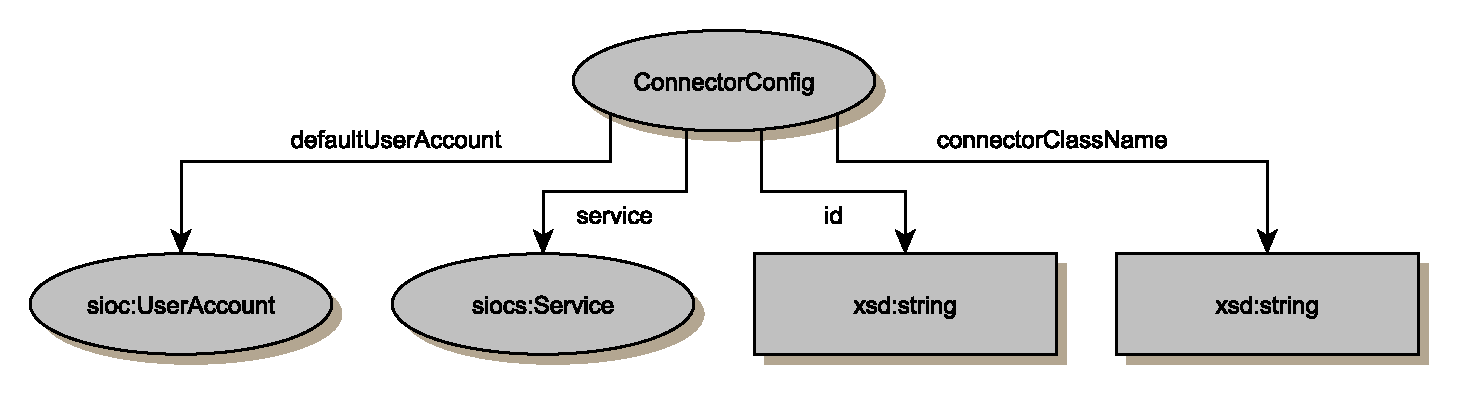
\includegraphics[
        width=\textwidth,
        keepaspectratio=true
    ]{assets/images/connector_config_ontology}
    \caption{Connector Config Ontology}
    \label{fig:uebersicht_conector_cfg}
\end{figure}

Aus diesem Grunde wurde für die Konfiguration eines Connectors die \emph{Connector Config Ontology} entwickelt. Abbildung \ref{fig:uebersicht_conector_cfg} zeigt diese Ontologie. Jeder Connector bekommt einen eindeutigen Bezeichner(kurz ID) um jeden diesen identifizieren zu können. Dies kann eine beliebige Zeichenkette sein. Um die korrekte Javaklasse des zu erstellenden Connectors benutzen zu können, wird der vollständige Klassenname, wie er zum Beispiel von \lstinline{object.class.getName()} zurückgegeben wird, in \texttt{connectorClassName} gespeichert. Für den Zugriff auf die Daten der SOC sind bei einiges APIs bestimmte Parameter wie die genaue Adresse des Servers notwendig. SIOC bietet hierzu ein eigenes Modul an, welches genau für solche Beschreibungen von Diensten die SIOC Ontologie erweitert. Eine kurze Beschreibung dieses Moduls und eine Erweiterung des selbigen für den Einsatz in SOCC befindet sich im Abschnitt \ref{ssub:services} und \ref{ssub:authorization}. Als Letztes braucht ein Connector noch einen vordefinierten Benutzer welcher als \texttt{defaultUserAccount} als SIOC UserAccount gespeichert wird. Dieser vordefinierte Benutzer erfüllt im Großen und Ganzen zwei Aufgaben. Als Erstes wird er für lesende Zugriffe der API auf die SOC genutzt, da hierzu ein einzelner Benutzer vollkommen ausreichend ist. Die zweite Aufgabe bezieht sich auf das stellvertretende Schreiben einzelner Benutzer. Nicht immer werden die dazu notwendigen Daten von den Benutzer zur Verfügung gestellt oder sind unbekannt. In diesem Fall wird der vordefinierte Benutzer genutzt und der Beitrag mit einem Vermerk zum original Autor über diesen geschrieben.


\subsubsection{Services} % (fold)
\label{ssub:services}

Wie eben schon beschrieben, existiert für SIOC ein Modul zur einfachen Modellierung von Diensten auf semantischer Ebene. Kernstück dieses Moduls ist die Klasse Service, wie auf Abbildung \ref{fig:uebersicht_sioc_services} zu sehen ist. Mit dieser Klasse kann durch eine Hand voll Eigenschaften ein Dienst beschrieben werden. Für diese Arbeit ist davon die wichtigste Eigenschaft \texttt{service\_endpoint}. Durch diese kann die Adresse festgelegt werden, unter dem ein bestimmter Dienst erreichbar ist. Gerade bei Plattformen die nicht an eine feste Adresse (Foren, Blogs, $\dots$) gebunden sind, ist diese Angabe unerlässlich. 

\begin{figure}[ht]
    \centering
    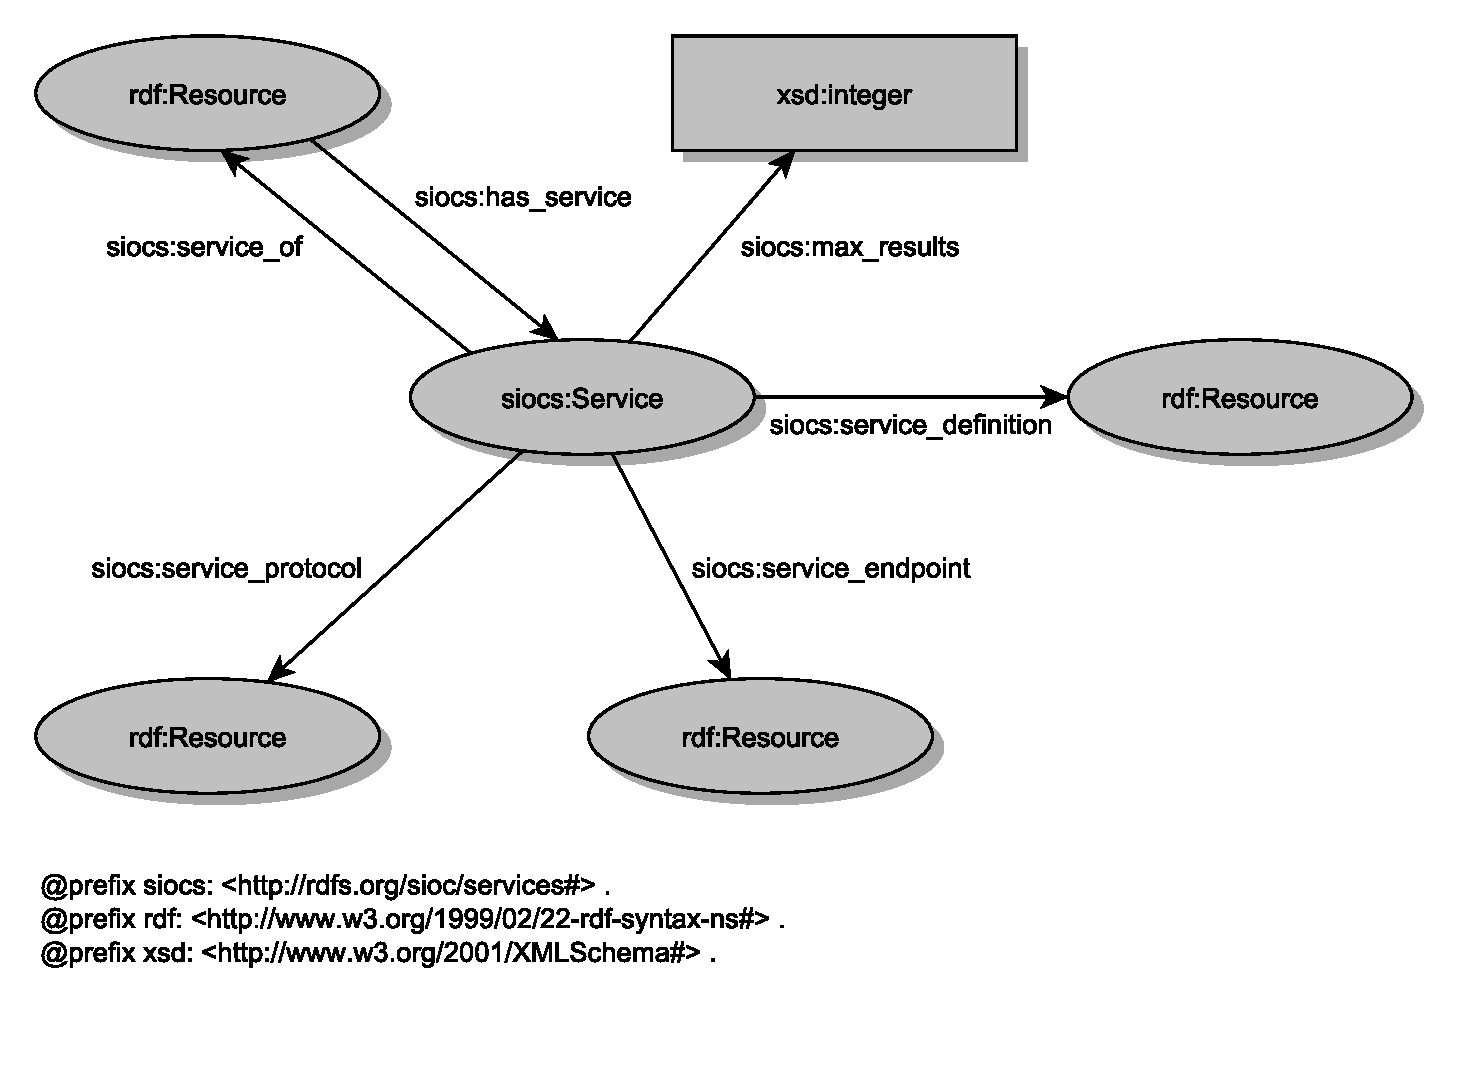
\includegraphics[
        width=0.7\textwidth,
        keepaspectratio=true
    ]{assets/images/sioc_services_ontology}
    \caption{SIOC Services Ontology}
    \label{fig:uebersicht_sioc_services}
\end{figure}

Die Eigenschaften \texttt{has\_service} und \texttt{service\_of} sind sind ideal zur Verbindung von einzelnen SIOC UserAccounts mit einem Service. Diese Verbindung hilft dabei für das stellvertretende Schreiben von Beiträgen schnell die passenden Benutzerdaten zu finden. Ebenfalls nützlich ist \texttt{max\_results}. Manche Dienste erlauben es nur eine maximale Anzahl an Ergebnissen pro Aufruf zurückgeben zu lassen. Da sich diese Anzahl über die Zeit ändern kann ist es nicht sinnvoll diese fest im Programm festzulegen, kann diese so im Nachhinein verändert werden. Für SOCC weniger interessant aber Vollständigkeit halber seien noch erwähnt \texttt{service\_protocol} zum Angeben des verwendeten Übertragungsprotokolls (REST\footnote{Representational State Transfer}, SOAP\footnote{Simple Object Access Protocol}, $\dots$) und \texttt{service\_definition} mit dem auf eine weiterführende Definition verwiesen werden kann.

% subsubsection services (end)

\subsubsection{UserAccounts} % (fold)
\label{ssub:useraccounts}

% subsubsection useraccounts (end)

\subsubsection{Autorisierung und Authentifizierung} % (fold)
\label{ssub:authentication}

Die Wahl für SIOC als Datenformat zu hat sich nach den ersten Tests als eine sehr gute Entscheidung herausgestellt. Mittels SIOC ließen die wichtigsten Daten aller untersuchten Plattformen in einer einheitlichen Form speichern. Die ersten Probleme traten erst auf, als es daran ging Daten für die Autorisierung (Feststellen ob jemand eine Handlung ausführen darf) beziehungsweise Authentifizierung (Feststellen ob jemand der ist, den er vorgibt zu sein) an den verschiedenen Programmierschnittstellen einen geeigneten Ort zu finden. Dazu musste aber erst festgestellt werden, welche verschiedenen Daten alle vorliegen können.

\medskip

\begin{description}
    \item[Username/Passwort] ist wohl eine der ersten und häufigsten Mechanismen, um den Zugriff sensibler Daten vor Dritten zu schützen. Das in Abschnitt \ref{sub:moodle_connector} beschriebene LMS Moodle, setzt zum Beispiel den Username und Password eines angemeldeten Benutzers zu Authentifizierung ein.
    
    \item[OAuth]\footnote{\url{http://oauth.net/}} stellt heutzutage den Standard der verwendeten Authentifizierungsmechanismen für hauptsächlich webbasierte API dar. Benutzer können so temporär Programmen den Zugriff auf ihre Daten erlauben und später wieder verbieten. Der aktuelle Standard stellt OAuth 2.0 dar und wird in dieser Version von den größten Seitenbetreibern wie Google, Facebook oder Microsoft eingesetzt\footnote{\url{http://en.wikipedia.org/wiki/OAuth\#List\_of\_OAuth\_service\_providers}}. Insgesamt sind für die Nutzung von OAuth vier Parameter wichtig. Für das Programm, dass Zugriff erhalten möchte sind die Parameter \emph{client\_id} und \emph{client\_secret} \cite{rfc6749}[S.\,8]. Sie weisen das Programm als autorisiert für die Benutzung der Schnittstelle aus. Soll nun beim Aufrufer einer von OAuth geschützten Funktion belegt werden ist ein sogenannter Accesstoken\cite{rfc6749}[S.\,9] nötig. Da dieser Accesstoken in der Regel nur eine bestimmte Zeit gültig ist, wird je nach Implementierung des Standards noch ein Refreshtoken mitgeliefert. Mit diesem Refreshtoken ist das Programm in der Lage ohne Zutun des Benutzers einen abgelaufen Accesstoken wieder zu aktivieren. Dies kann beliebig oft wiederholt werden, bis der Benutzer beide Token für ungültig erklärt.
    \todo[inline]{vll. noch OAuth 1.0(a) einbauen}
    
    \item[API Schlüssel] sind eine dritte Möglichkeit Programmen Zugriff auf eine API zu gewähren. Der API Schlüssel entspricht ungefähr einer Kombination von client\_id und client\_secret von OAuth. Dieser Schlüssel schaltet in der Regel nicht den Zugriff auf persönliche Daten von Benutzer frei. Hier ist noch ein weiterer Mechanismus wie die Verwendung von einem Usernamen und Passwort nötig. Die in Abschnitt \ref{sub:youtube_connector}  beschriebene Google Youtube API hierzu ein gutes Beispiel.
\end{description}

\medskip

\begin{figure}[h]
    \centering
    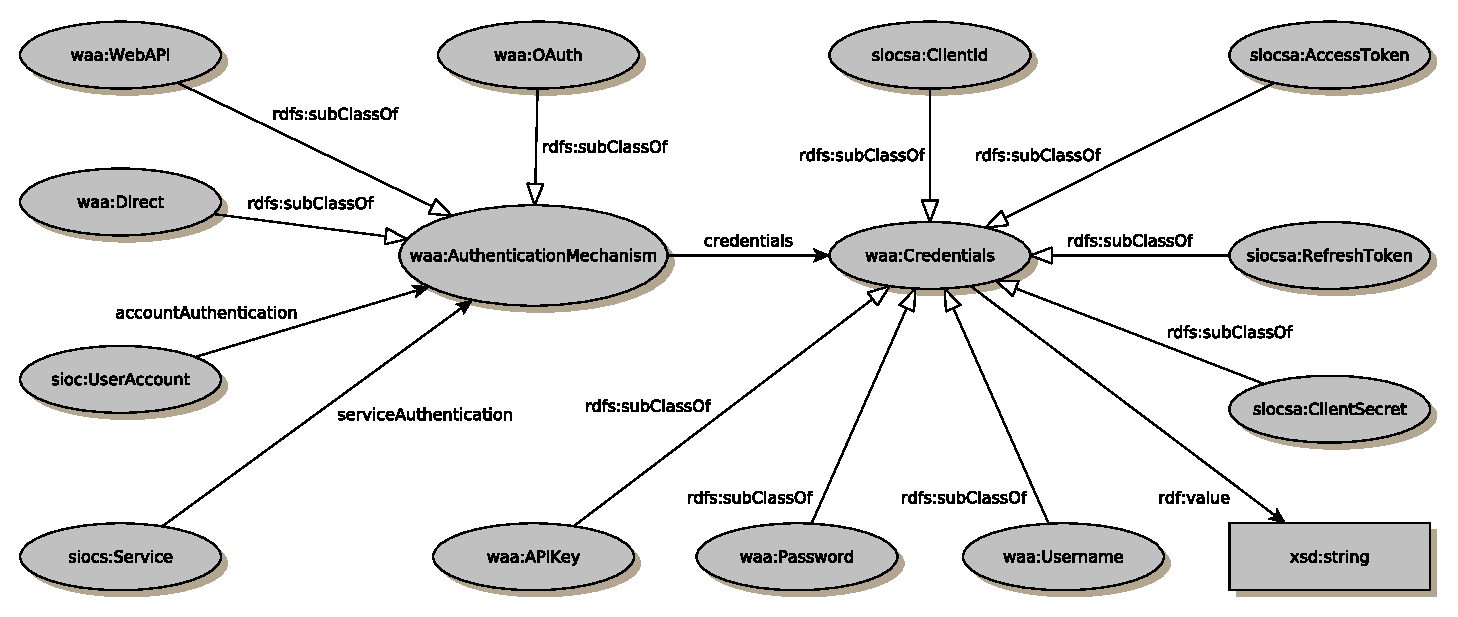
\includegraphics[
        width=\textwidth,
        keepaspectratio=true
    ]{assets/images/sioc_services_authentication}
    \caption{SIOC Services Authentication Ontology}
    \label{fig:uebersicht_sioc_services_authentication}
\end{figure}

Neben diesen drei Mechanismen wäre noch der Vollständigkeit halber die HTTP-Authentifizierung zu nennen. Hierbei handelt es ich um eine Form des Username/Passwort Verfahrens, welches auf das HTTP Protokoll aufsetzt. Für einfachen Webseiten ist dies ein unkomplizierte Art die Datei vor fremden Zugriffen zu schützten. Für aktuelle öffentliche APIs ist diese Form der Authentifizierung nicht mehr Stand der Technik.

\medskip

Die Suche nach einer bestehen Ontologie, welche zusammen mit SIOC verwendet werden könnte, gestaltete sich als sehr schwierig. Ein Großteil der Ontologien in diese Richtung befasst sich eher mit dem Thema der Autorisierung wie Zugriffssteuerungsliste wie zum Beispiel die \emph{Web Access Control List} \cite{Hollenbach2009}. Nicht desto trotz existiert auch eine Authentifizierung Ontologie. Die \emph{Authentication Ontology}\footnote{\url{http://omnivoke.kmi.open.ac.uk/authentication/}} des \emph{OmniVoke}\footnote{\url{http://omnivoke.kmi.open.ac.uk/framework/}} ist für die geforderten Zwecke das ideale Werkzeug. 

% subsubsection authorization (end)

% subsection konfiguration (end)

\subsection{Aufbau eines Connectors} % (fold)
\label{sub:connector_aufbau}

\begin{figure}[ht]
    \centering
    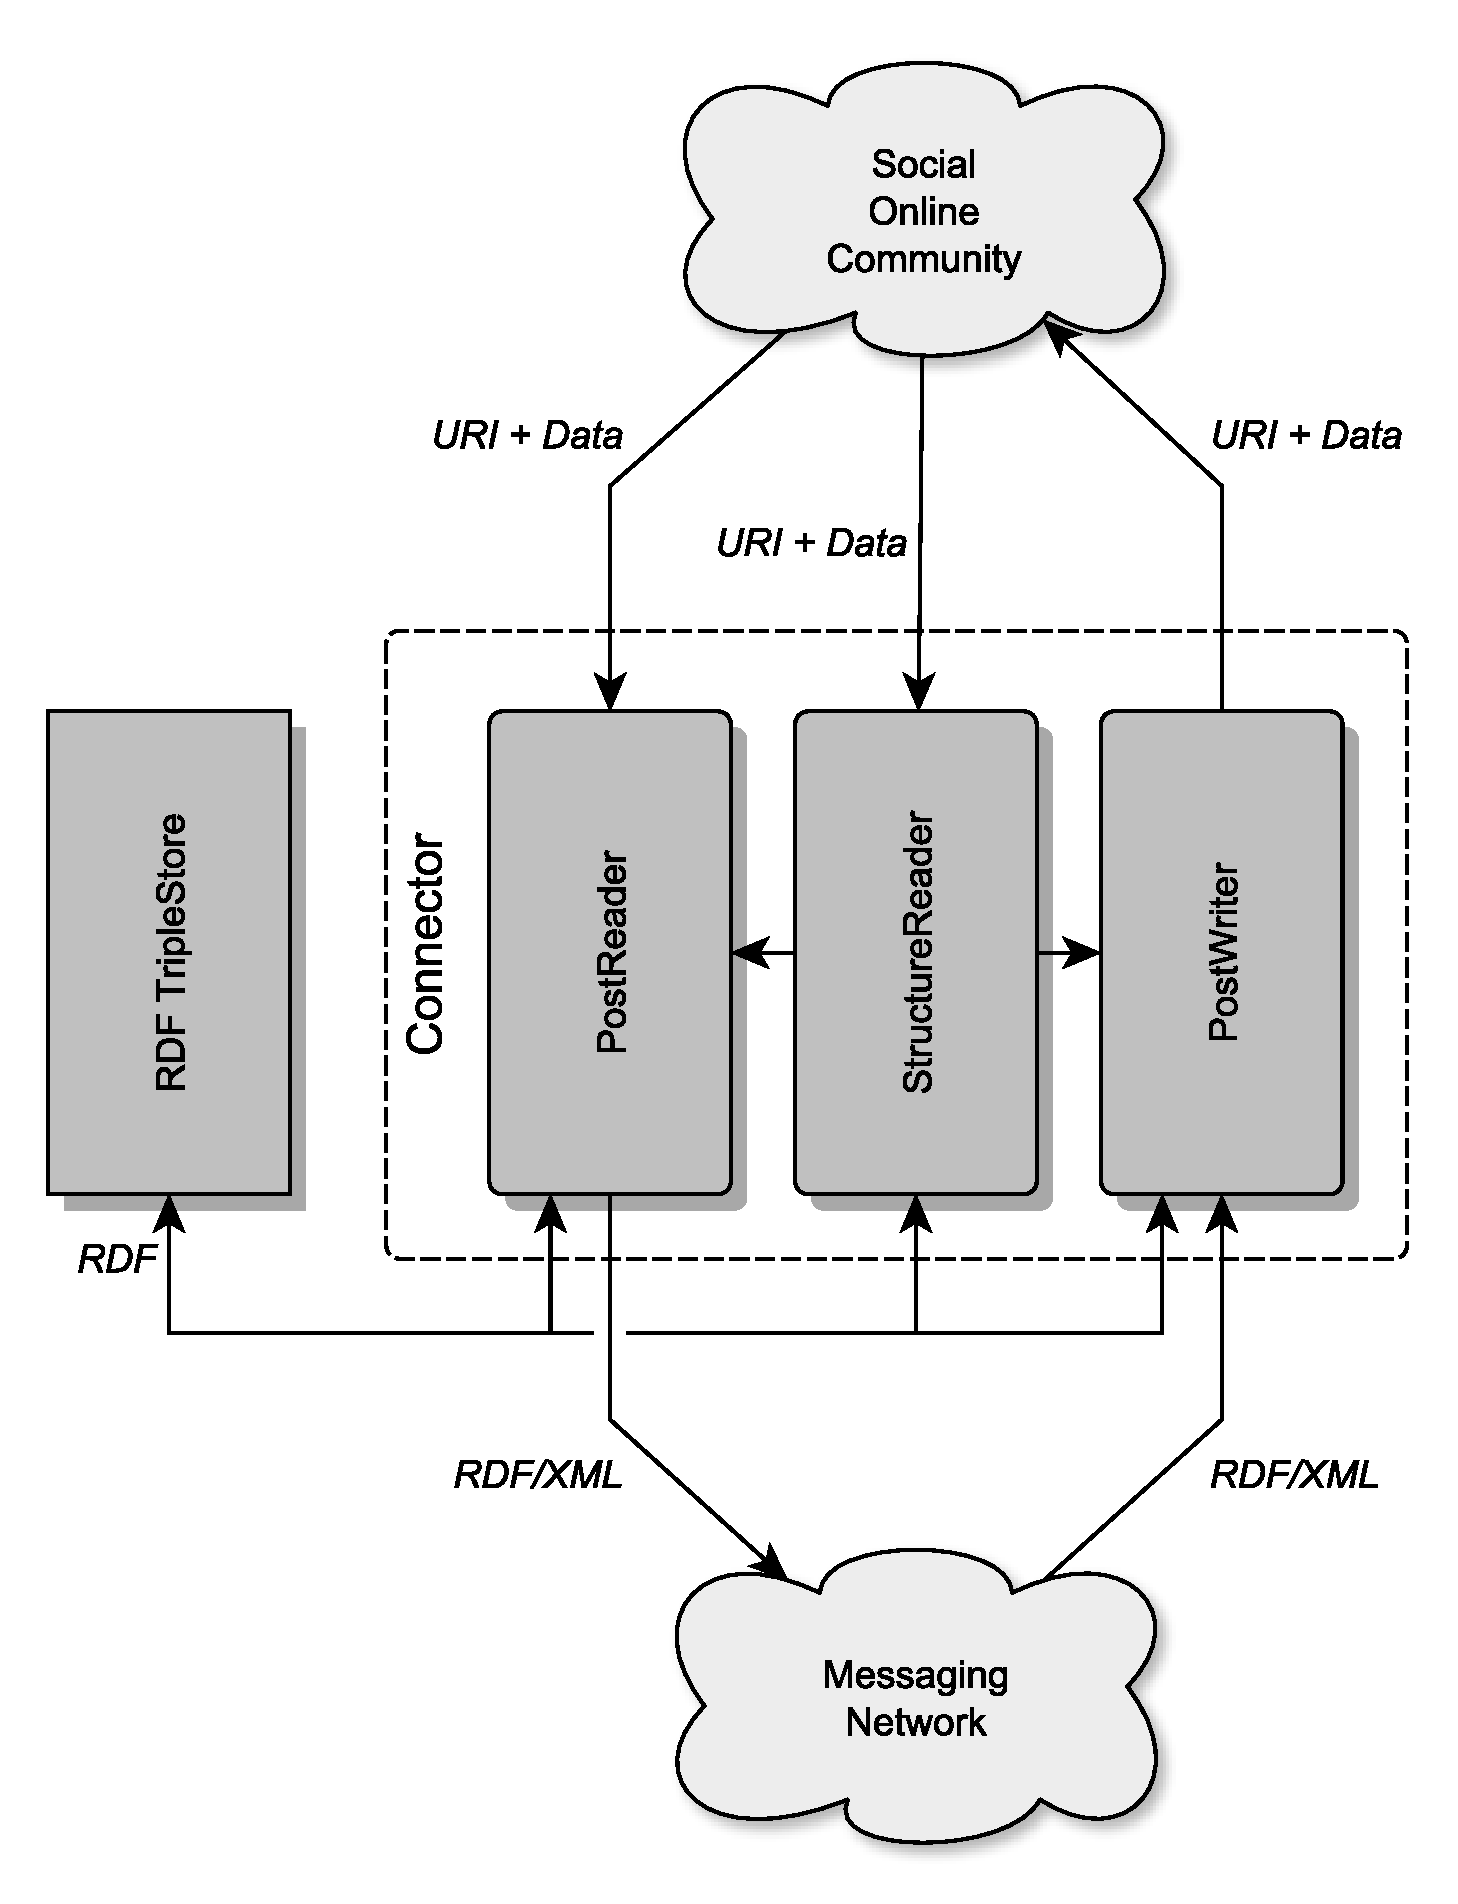
\includegraphics[
        width=0.5\textwidth,
        keepaspectratio=true
    ]{assets/images/socc_connector_overview}
    \caption{Übersicht der Komponenten der SOCC}
    \label{fig:uebersicht_socc}
\end{figure}

\subsubsection{ClientManager} % (fold)
\label{ssub:clientmanager}

% subsubsection clientmanager (end)

\subsubsection{StructureReader} % (fold)
\label{ssub:structurereader}

\begin{wrapfigure}[10]{r}{7cm}
    \centering
    \includegraphics[
        width=5cm,
        keepaspectratio=true,
        clip=true,
        trim= 0 126 456 326
    ]
    {assets/images/uml_iconnector.png}
    \caption{StructurReader}
    \label{fig:uml_structure_reader}
\end{wrapfigure}
Um auf Informationen über die Struktur von Foren, sozialen Netzwerken und so weiter im SIOC Format zugreifen zu können, implementiert jeder Connector dazu einen StructureReader. Die Struktur lässt sich, wie im Abschnitt \ref{sec:social_online_community_connectors} gezeigt, durch die SIOC Klassen \emph{Site} und \emph{Container} (und Unterklassen davon) beschrieben. Um auf diese Struktur zugreifen zu können, enthält die StructureReader Schnittstelle mehrere Methode (Siehe Abbildung \ref{fig:uml_structure_reader}). \wrapfill

\begin{description}
    \item[\texttt{getSite()}] ist eine Methode, welche die Beschreibung einer Seite (Forum, Blog, soziales Netzwerk) als SIOC Site Objekt zurücklieft. Dies wird relativ häufig um die Zugehörigkeit einiger Objekte durch einen Link zu dieser Seite zu verdeutlichen. Dies kann bei einigen APIs nützlich sein, da dort manchmal keine Information zum \emph{Container} eines Beitrags mitgeliefert werden, über den man sonst eine Beziehung zwischen Seite und Beitrag herstellen könnte.

    \item[\texttt{getContainer(URI)}] ist dazu gedacht die Information eines einzelnen Containers erhalten der sich hinter eine URI verbirgt.

    \item[\texttt{listContainer(...)}] sind Methoden welche für den die Auflisten aller Container einer Seite zur Verfügung stehen. Die Methode ohne Parameter listet alle Container auf der ersten Ebene auf. Dies könnten zum Beispiel alle Kurse auf einen Canvas LMS Seite oder alle Gruppen auf Facebook sein. Die zweite Methode mit URI Parameter gibt eine Liste alle Container, welche den Container hinter der übergeben URI als Elternteil haben, zurück. Als Beispiel wären alle Themen innerhalb eines Forums zu nennen.

    \item[\texttt{hasChildContainer(URI)}] überprüft ob der Container hinter einer URI überhaupt weitere Container als Kinder besitzt. Diese Methode wird dazu eingesetzt, um vorab zu testen, ob der Aufruf von \texttt{listContainer(URI)} das gewünschte Ergebnis liefert oder ein Fehler auftritt. 
\end{description}

% subsubsection structurereader (end)

\subsubsection{PostReader} % (fold)
\label{ssub:postreader}

\begin{wrapfigure}{r}{7cm}
\centering
\includegraphics[
width=6cm,
keepaspectratio=true,
clip=true,
trim= 220 144 220 344
]{assets/images/uml_iconnector.png}
\caption{PostReader}
\end{wrapfigure}

Der \texttt{PostReader} dient als Schnittstelle, um auf geschriebene Beitrage innerhalb eines Containers oder die Kommentare auf eines Beitrags zuzugreifen. Die Methode \texttt{hasPosts(URI)} ist nur zur Überprüfung ob ein Container oder ein Beitrag hinter einer URI weiter Beiträge enthält die gelesen werden können. Um einen einzelnen Beitrag anhand seiner URI lesen zu können kann die Methode \texttt{getPost(URI)}  genutzt werden. Sei liefert dann den Beitrag SIOC Post Objekt zurück beziehungsweise einen Fehler, falls der Beitrag nicht mit diesem Connector gelesen werden kann. Die wichtigste Methode dahingegen ist \texttt{pollPosts(URI, Date, int)}. Insgesamt können dieser Methode drei Parameter übergeben werden. Der Erste ist eine URI die den Ort angibt von der alle Beiträge gelesen werden können. Mit dem zweiten Parameter kann ein Zeitpunkt angegeben werden, ab dem ein zu lesender Beitrag geschrieben sein muss. Alle Beiträge die vor diesem Zeitpunkt erstellt wurden, werden nicht zurück gegeben. Der letzte Parameter gibt eine obere Schranke an wie viele Beiträge maximal pro Aufruf dieser Methode gelesen werden dürfen.

% subsubsection postreader (end)

\subsubsection{PostWriter} % (fold)
\label{ssub:postwriter}

In Abbildung \ref{fig:postwriter_sequenzdiagramm} ist ein Sequenzdiagramm der PostWriter Komponente zu sehen. Dort ist visualisiert, welche Schritte für das stellvertretende Schreiben von Beiträgen eines Benutzers unternommen werden müssen. Soll nun ein Beitrag in einer SOC geschrieben werden, wird die Methode \texttt{writePost(URI, String, Syntax)} mit dem Zielort als URI, dem Beitrag als serialisiertes RDF Objekt und dem verwendeten Serialisierungsformates aufgerufen. Begonnen wird damit, dass als erstes nach einem UserAccount für den Service des aktuellen Connectors des Beitragautors gesucht. Im Idealfall befindet sich für den UserAccount des Beitragsautors ein Link zu seiner FOAF Person und von ein weiterer Link zum UserAccount für den aktuellen Service. Mit diesem UserAccount kann dann vom ClientManager ein Clientobjekt für die verwendete API angefordert werden. Sollte die Suche negativ verlaufen, steht der vordefinierte Client zur Verfügung. Mit diesem Client, ob mit der des Autors oder dem Vordefinierten, wird im letzten Schritt der Beitrag im von der API verwendeten Format in die SOC geschrieben.
\begin{figure}[h]
\centering
\includegraphics[
width=\textwidth,
keepaspectratio=true,
clip=true,
trim= 90 200 220 75
]{assets/images/postwriter_sequencediagram}
\caption{PostWriter Sequenzdiagramm}
\label{fig:postwriter_sequenzdiagramm}
\end{figure}

% subsubsection postwriter (end)

% subsection connector_aufbau (end)

% section social_online_community_connectors (end)

\section{SOCC-Camel} % (fold)
\label{sec:socc_camel}

\begin{figure}[h]
     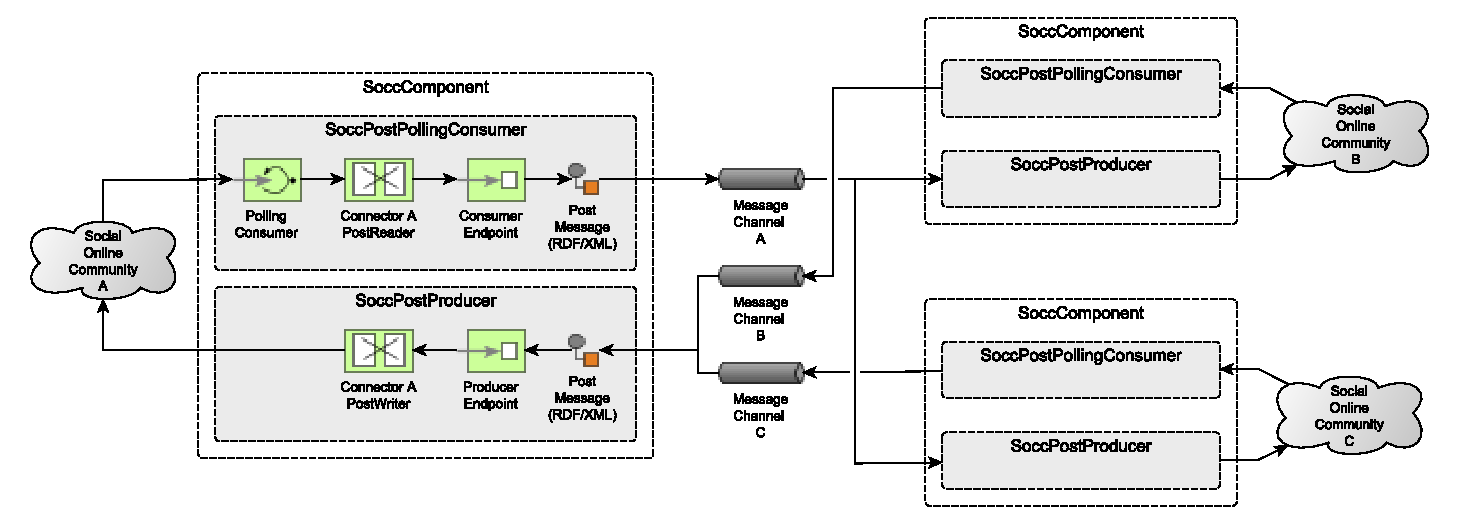
\includegraphics[
        width=\textwidth,
        keepaspectratio=true
    ]{assets/images/socc_camel_overview}
    \caption{Übersicht des Apache Camel Moduls Socc-Camel}
    \label{fig:uebersicht_socc_camel}
\end{figure}

\subsection{SoccComponent} % (fold)
\label{sub:socccomponent}

% subsection socccomponent (end)

\subsection{SoccPostPollingConsumer} % (fold)
\label{sub:soccpostpollingconsumer}

% subsection soccpostpollingconsumer (end)

\subsection{SoccPostProducer} % (fold)
\label{sub:soccpostproducer}

% subsection soccpostproducer (end)

% section socc_camel (end)

% chapter eigener_ansatz (end)

		%!TEX root = ../thesis.tex

\chapter{Implementierung und Evaluation} % (fold)
\label{cha:implementierung_und_evaluation}

\todo[inline]{Auf die verschiedenen Klassen von Facebook und Co eingehen, REST, SOAP, OAUTH, Client/Passwort, Art der Plattforn, Forum, OSN, Videoplatform}

\section{Verwendete Programme und Bibliotheken} % (fold)
\label{sec:verwendete_bibliotheken_und_programme}

An dieser Stelle soll noch kurz auf zusätzliche Programm und Bibliotheken eingegangen werden, die für die Entwicklung der einzelnen Connectoren hilfreich waren. 

\subsection{Apache Maven} % (fold)
\label{sub:apache_maven}

Für die Entwicklung der Programme und Bibliotheken dieser Arbeit wurde das Buil-Management Programm \texttt{Maven}\footnote{http://maven.apache.org/} von Apache eingesetzt. Mit diesem ist es auf einfache Art möglich Java-Programme zu verwalten und zu erstellen. So ist nur mit einer einzigen XML-Datei (\texttt{pom.xml}) die Abhängigkeiten festzulegen, das Programm zu kompilieren, zu testen und es auszuliefern. Maven schreibt eine feste Ordnerstruktur für ein Projekt vor wie der Produktivquellcode, dafür nötige Ressource (Bilder, Teste,\dots) und der Code zum Testen geordnet werden sollen. Die Abhängigkeiten werden automatisch aus zentralen Repositories heruntergeladen und ins Projekt eingebunden. So muss dies nicht immer von Handgeschehen und spart so Arbeit.

% subsection apache_maven (end)

\subsection{RDF2Go} % (fold)
\label{sub:rdf2go}

% subsection rdf2go (end)

% section verwendete_bibliotheken_und_programme (end)

\section{Implementierung der Connectoren} % (fold)
\label{sec:implementierung_der_connectoren}

An dieser Stelle soll beschrieben werden wie Connectoren für die in Abschnitt \ref{sec:lernplattformen_und_soziale_online_netzwerke} vorgestellten Plattformen implementiert werden können. Dafür wird darauf eingegangen mit welcher Art von API auf die Daten der einzelnen Plattformen zugegriffen werden und wie man deren Datenstruktur in SIOC abbilden kann. Ebenfalls werden auftretende Probleme und wenn möglich deren Lösung gezeigt.

Innerhalb der Beschreibungen des Mappings nach SIOC werden zur besseren Übersicht und einfacheren Lesbarkeit Platzhalt für einige URIs benutzt. Welche Platzhalten dies sind und für welche URI sie stehen ist aus Tabelle \ref{tbl:platzhalter_fuer_sioc_mapping} zu entnehmen.
\begin{table}[ht]
    \centering
    \caption{Allgemeine Platzhalter und deren Beschreibung für das Mapping nach SIOC}
    \begin{tabular}{l|p{11cm}}
        \textbf{Platzhalter} & \textbf{Bedeutung} \\ 
        \hline
        \texttt{\{serviceUri\}} & URI für einen Service \\
        \texttt{\{userAccountUri\}} & URI für einen UserAccount \\
        \texttt{\{siteUri\}} & URI für eine Site \\
        \texttt{\{forumUri\}} & URI für ein Forum \\
        \texttt{\{threadUri\}} & URI für ein Thread \\
        \texttt{\{postUri\}} & URI für ein Post \\
        \texttt{\{rootUri\}} & Die WurzelUri einer SOC. Für Facebook wäre dies zum Beispiel \texttt{https://www.facebook.com}
    \end{tabular}
    \label{tbl:platzhalter_fuer_sioc_mapping}
\end{table}

\\subsection{Allgemeine Probleme} % (fold)
\label{sub:allgemeine_probleme}

% subsection allgemeine_probleme (end)

\subsection{Moodle} % (fold)
\label{sub:moodle_connector}

% \begin{itemize}
%     \item Eingebaute REST Schnittstelle, aber kein Lesen von Beiträgen
%     \item WebService Plugin MoodleWS (REST oder SOAP)
%     \begin{itemize}
%         \item https://github.com/patrickpollet/moodlews
%         \item ClientAPI existieren von selber Autor
%         \item REST defekt, kein schreiben von Beiträgen möglich
%         \item SOAP funktioniert mehr oder weniger
%         \item Verschluckt Fehlermeldungen
%         \item kein lesen einzelner Posts/Threads/Foren
%         \item SOAP ClientAPI neu generieren, weil vorhandene nicht mit 2.4 funktioniert.
%         \item Username/Password + Session Token/Id
%         \item “Use an auto generated wsdl” -> No
%         \item schreiben von neuen Beitrag direkt in thread nur als Antwort auf ersten Beitrag möglich
%         \item Rückgabe aller Beiträge in einem Objekt
%     \end{itemize}
% \end{itemize}

\subsubsection{Moodle Webservice API} % (fold)
\label{ssub:moodle_webservice}

Moodle bringt von Haus aus schon eine Webservice-Schnittstelle für einen Zugriff auf seine Daten mit. Diese API unterstützt dabei Protokolle für REST, SOAP und oder XML-RPC\footnote{\url{http://xmlrpc.scripting.com/}}. Mit ihr können Kurse, Foren und deren Threads (in Moodle Discussion Topics genannt), Benutzerprofile, Gruppen und viele andere Ressourcen ausgelesen oder geschrieben werden. Leider gilt dies nicht für Beiträge innerhalb von Foren Threads. Die aktuelle Version (Beim verfassen dieser Arbeit war dies 2.5.1) erlaubt es nicht Beiträge weder zu lesen noch zu schreiben.

Doch existiert ein Plugin für Moodle, dass auf dieser Webservice API aufbaut und erweitert - \emph{MoodleWS}\footnote{\url{https://github.com/patrickpollet/moodlews}}. MoodleWS bietet den Zugriff über REST und SOAP, wobei bei der Verwendung von REST JSON als Datenformat verwendet wird und nicht XML wie mit SOAP. Mit diesem Plugin ist ein Programm nun auch in der Lage Beiträge aus Threads zu lesen. Die REST-Schnittstelle hat aber noch eine paar Fehler und so können damit noch keine neuen Beiträge geschrieben werden. Mit SOAP ist dies aber problemlos möglich.

Für die Benutzung der muss sich ein Client mit dem Benutzernamen und Passwort eines vorhandenen Benutzers anmelden. Ist dies erfolgreich, bekommt der Client einen zufällig ID und einen Sitzungsschlüssel die er bei jeder Abfrage angeben muss. Dieser Sitzungsschlüssel ist nur eine begrenzte Zeit gültig, so kann es passieren, dass eine Operation fehlschlägt und der Client sich neu anmelden muss.

Für die Verwendung der API in Java wird auch eine Bibliothek moodle\_ksoap2\footnote{\url{https://github.com/patrickpollet/moodlews\_ksoap2}} zur Verfügung gestellt. Sie abstrahiert komplett das SOAP-Protokoll im Hintergrund und enthält für alle Moodle-Ressource Java-Klassen und Methoden für den Zugriff. Bevor moodlews\_ksoap2 benutzt werden kann, ist darauf zu achten in Moodle unter \enquote{Site administration}, \enquote{Development}, \enquote {OK Tech Webservices ( aka wspp)} die Einstellung \enquote{Use an auto generated wsdl} auszuschalten, da es sonst zu Problemen mit moodlws\_ksoap2 kommen kann.

\begin{lstlisting}[
    caption={MoodleWS mit moodlews\_ksoap2: Lesebeispiel}\label{lst:moodlews_java_beispiel},
    captionpos=t]
Mdl_soapserverBindingStub client = new Mdl_soapserverBindingStub(
        MOODLE_URI + "/wspp/service_pp2.php",
        MOODLE_URI + "/wspp/wsdl2",
        false );

LoginReturn loginReturn = client.login(username, password);

ForumRecord[] forumRecords = client.get_all_forums(
        loginReturn.getClient(),
        loginReturn.getSessionKey(),
        "",
        "" );

for(ForumRecord forum : forumRecords){
    System.out.println(forum.getId() + " " + Forum.getName());
}
\end{lstlisting}

Wie in der ersten Zeile von Listing \ref{lst:moodlews_java_beispiel} zu sehen wird als ist der Client eine Objekt der Klasse \texttt{Mdl\_soapserverBindingStub} aus moodlews\_ksoap2. Dem Konstruktor wird die URI auf die Datei \enquote{service\_pp2.php} (Zeile 3) und der XML-Namespace der WSDL-Datei des MoodleWS-Plugins übergeben. Das dritte Argument besagt, ob der Client im Debugmodus laufen und mehr Logging-Ausgaben macht über die einzelnen internen Abläufe ausgeben soll. In Zeile 6 meldet sich der Client mit einen Benutzernamen und einem Passwort bei MoodleWS an und bekommt ein Objekt der Klasse \texttt{LoginResult} mit der oben angesprochenen ID für den Client und einen Sitzungsschlüssel zurück. Mit der Methode \texttt{get\_all\_forums(\dots)} können nun ein Array mit allen Foren angefordert werden, auf die der angemeldete Benutzer Zugriff hat. Die ersten zwei Argumente dieser Methode sind die ID des Clients und der Sitzungsschlüssel. Mit den letzten zwei Argumenten kann das Ergebnis gefiltert werden. Dazu wird als erstes ein Spaltenname aus der Foren-Tabelle der Moodle-Datenbank angeben und als zweites welcher Wert dieser haben soll. Am Ende werden dann alle Ergebnisse mit der ID und Name des Forums ausgegeben.

\begin{lstlisting}[
    caption={MoodleWS mit moodlews\_ksoap2: Beitrag schreiben}\label{lst:moodlews_beitrag schreiben},
    captionpos=t]
ForumPostDatum postDatum = new ForumPostDatum(client
                    .getBindingStub()
                    .getNAMESPACE());

postDatum.setMessage("War kam bei der Aufgabe raus?");
postDatum.setSubject("Aufgabe 2.1");

client.forum_add_reply(
        client.getAuthClient(),
        client.getSessionKey(),
        postId,
        postDatum);
\end{lstlisting}

Beiträge können nur als Kommentare geschrieben werden und dessen ID bekannt sein. Alle Daten für den Beitrag werden in einem Objekt der Klasse \texttt{ForumPostDatum} gespeichert, wie in der ersten Zeile des Listings \ref{lst:moodlews_beitrag schreiben} zu sehen ist. Das Argument ist der beim Client angegebene XML-Namespace der WDSL-Datei. Als Daten können wie in Zeile 5 und 6 nur eine Nachricht (Message) und ein Thema (Subject) übergeben werden. Dieses Objekt wird dann an die Methode \texttt{forum\_add\_reply} mit der ID des Clients, dem Sitzungsschlüssel und der ID des Beitrags wohin geschrieben werden soll übergeben und an Moodle übertragen.s

% subsubsection moodle_webservice (end)

\subsubsection{Moodle Mapping nach SIOC} % (fold)
\label{ssub:moodle_mapping_nach_sioc}



% subsubsection moodle_mapping_nach_sioc (end)

\subsubsection{Besonderheiten bei der Implementierung des MoodleConnectors} % (fold)
\label{ssub:herausforderungen_bei_der_implementierung_des_moodleconnectors}

Der Connector für Moodle war wohl einer der herausforderndsten bei der Implementieren von allen fünf Connectoren. Nicht nur weil erst nach mehreren Test sich herausstellte, dass die favorisierte REST-Schnittstelle von MoodleWS kein schreiben von Beiträgen möglich macht sondern dass auch die Java-Bibliothek moodlews\_ksoap2 so ihre kleinen Eigenheiten hat. 

Zuerst mussten die Klasse für moodlews\_ksoap2 komplett neu generiert werden. In der Dokumentation wird beschrieben, dass dieser Schritt nötig ist, wenn sich an der WSDL-Datei von MoodleWS was geändert hat. Der passende Generator wird vom Entwickler gleich mitgeliefert und ist mit dem folgenden Befehl schnell bewerkstelligt.

\begin{lstlisting}[
    caption={Neugenerierung von moodlews\_ksoap2}\label{lst:neugenerierung_moodlews_ksoap2},
    captionpos=t]
    java  org.ksoap2.wsdl.WSDL2ksoap -p de.m0ep.moodlews.soap -o /tmp http://localhost/moodle/wspp/wsdl_pp2.php
\end{lstlisting}

Mit dem Parameter \enquote{-p} wir das Java-Package für die Java-Klassen festgelegt und mit \enquote{-o} der Ordner in dem die Klassen geschrieben werden. Die URI am Ende gibt den Pfad zur Datei \enquote{wsdl\_pp2.php} vom MoodleWS-Plugin. Diese ist dann an die jeweilige Moodle Instanz anzupassen.

Eine sehr nervende Eigenheit von moodlews\_ksoap2 ist die Tatsache, dass Java-Exceptions und Gründe für Fehler gerne verschluckt und nicht weitergegeben werden. So ist es zum Beispiel nicht möglich zu wissen ob eine Operation aufgrund eines Netzwerkfehlers, eines abgelaufenen Sitzungsschlüssels oder falschen Daten fehlschlug. Aus diesem Grund wurde der Client von moodlews\_ksoap2 für den ClientManager (siehe Abschnitt \ref{sub:clientmanager}) in eine extra Klasse \texttt{Moodle2ClientWrapper} gepackt und um Mechanismen zur Fehlererkennung und Wiederherstellung erweitert. Alle Funktionsaufrufe des Clients wie \texttt{get\_all\_forums(\dots)} werden dazu zuerst in die Methode \texttt{call} eines Objekts des Java-Interfaces \texttt{Callable<V>} verpackt, so dass diese Funktion, ohne zu wissen um welche es sich genau handelt, mehrfach aufrufen werden kann. Diese Objekt wird dann an die Methode \texttt{callMethod(\dots)} der Klasse \texttt{Moodle2ClientWrapper} übergeben. Diese Methode ruft dann zuerst die \texttt{call()} Methode des Callabel-Objekts und prüft ob ein gültiges Ergebnis zurückgegeben wurde. Dies ist der Fall wenn es ungleich \texttt{null} ist. Ist dies nicht der Fall, wird geschaut ob die Moodleinstanz erreichbar ist. Sollte hier alles in Ordnung sein, muss geschaut werden ob der Sitzungsschlüssel abgelaufen ist. Als Test reicht hier es hier aus, ob die Methode \texttt{get\_my\_id(\dots)} des moodlews\_ksoap2 Clients eine Zahl ungleich 0 (Null) zurück gibt. Diese liefert die ID des aktuell angemeldeten Benutzers zurück und im Fehlerfall ist dieser gleich 0. Ist dieser Test positiv, also der Sitzungsschlüssel abgelaufen, wird versucht sich neu anzumelden und die Anfrage erneut ausgeführt.

Eine Funktion mit der nur ein Beitrag mit einer bestimmten ID abgefragt werden könnte fehlt ebenfalls. Wenn nur ein Beitrag geladen werden soll, müssen zunächst alle innerhalb des selben Threads angefordert und diese nach dem passenden Beitrag durch werden. 

Ebenfalls ungewöhnlich ist der Inhalt der Klasse \texttt{ForumDiscussionRecord}. Normalerweise würde mit erwarten, dass die Methode \texttt{getId()} die ID des Diskussionsthread zurück geben wird. Doch stattdessen entspricht der Wert der ID des ersten Beitrags dieses Threads. An die richtige ID kommt man erst rann, wenn man sich mit der Methode \texttt{getPost()} ein Objekt des ersten Beitrags und darin den Rückgabewert von \texttt{getDiscussion()} benutzt.

% subsubsection herausforderungen_bei_der_implementierung_des_moodleconnectors (end)

% subsection moodle_connector (end)

\subsection{Facebook} % (fold)
\label{sub:facebook_connector}

% \begin{itemize}
%     \item REST API + JSON
%     \item keine offizielle Java API für Desktop -> Web + Mobile only
%     \item GraphAPI, Facebook Query Language
%     \item OAuth 2.x
%     \begin{itemize}
%         \item kein Refreshtoken
%         \item Token Haltbarkeit 2h (2 Monate, wen extended)
%         \item token nur über webbrowser
%     \end{itemize}
%     \item RestFB alternative Java API für die REST Schnittstelle der GraphAPI
%     \item Typ der zurückgelieferten Daten nicht anhand der URI erkennbar, häufig erst durch Angabe von \emph{metadata=1}
%     \item beim herunterladen einzelner Posts nicht immer erkennbar wo sie geschrieben wurden
% \end{itemize}

\subsubsection{Facebook Graph API} % (fold)
\label{ssub:facebook_graph_api}

Die primäre Weg an die von Facebook gespeicherten Daten zu gelangen, geht über die \emph{Graph API}\footnote{Graph API Dokumentation:  \url{https://developers.facebook.com/docs/reference/api}}. Sie erlaubt einen REST basierten Zugriff auf den von Facebook sogenannten \emph{Social Graph} \cite{FacebookGraphAPI}. Dieser Graph enthält alle Beziehungen die ein Person auf Facebook zwischen anderen Personen, Gruppen, Seiten, Beiträge, Fotos und so weiter besitzt. Der einfachste Weg zum Kennenlernen der Graph API ist der \emph{Graph API Explorer}\footnote{Graph API Explorer: \url{https://developers.facebook.com/tools/explorer}}. Er ist eine Onlineanwendung REST-Abfragen an die Graph API schnell ausprobiert und das Ergebnis begutachtet werden kann.

Jede Ressource im Social Graph von Facebook hat seine eigen, eindeutige ID. Wegen diesem Merkmal besteht eine URI für den REST-Zugriff nur aus \texttt{https://graph.facebook.com/} gefolgt von der ID und optionalen Parametern. Dies macht die Form der URIs zwar sehr einheitlich, aber es ist so unmöglich anhand der URI herauszufinden welcher Typ von Ressource sich dahinter befindet. Dies widerspricht zwar nicht die am Anfang von Kapitel \ref{cha:eigener_ansatz_social_online_community_connectors_socc_} beschreiben Prinzipien von Berners-Lee macht aber die spätere Verarbeitung etwas komplizierter. 

\paragraph{Graph API Datenformat} % (fold)
\label{par:graph_api_datenformat}

Also Datenformat setzt Facebook mit der Graph API auf das unter Webanwendungen weit verbreitete JSON. Neben den eigentlichen Daten enthalten Ressourcen noch Verbindungen zu anderen Ressourcen. Diese Verbindungen werden \enquote{Connections} genannt. Um zu lesen welche Connections eine Ressource besitzt muss bei der Abfrage der Parameter \texttt{metadata=1} angehängt werden. Ist die geschehen enthalten die JSON Daten einen neuen Eintrag \texttt{metadata} und darin unter dem Eintrag \texttt{connections} eine Liste der vorhandenen Connections. Die wichtigsten Connections für diese Arbeit sind \texttt{feed}und \texttt{comments}. Die Connection \texttt{feed} sagt über die Ressource aus, dass sie eine Liste von Beiträgen enthält. Das könnten zum Beispiel die Wall einer Person oder die einer Gruppe sein. Dahingegen zeigt die Connection \texttt{comments}, dass die betreffende Ressource Kommentare enthält und auch kommentiert werden kann. Um die Beiträge eines Feeds lesen zu können, muss nur die ÜRI zu der Ressource mit den Pfad \texttt{/feed} erweitert werden: \texttt{http:/graph.facebook.com/me/feed}. Die ID \texttt{me} ist dabei ein spezielle ID die sich auf den aktuell angemeldete Benutzer bezieht. Möchte man nun nicht alle Daten einer Ressource abfragen sondern zum Beispiel nur den Name und das Datum der letzten Änderung, kann der Parameter \texttt{fields} für die URI eingesetzt werden. Als Wert wird dann eine Liste mit den Namen der gesuchten Daten angegeben, wobei jeder Name durch ein Komma getrennt wird. 

% paragraph graph_api_datenformat (end)

\paragraph{Facebook Login} % (fold)
\label{par:facebook_login}

Die Graph API verwendet zur Autorisierung der Anfragen OAuth 2.0 auch \emph{Facebook Login}\footnote{Facebook Login: \url{https://developers.facebook.com/docs/facebook-login/}} genannt. Accesstoken gelten bei Facebook nur für zwei Stunden. Es ist aber möglich einen sogenannten \emph{Extended Accesstoken}\footnote{Graph API Accesstokens: \url{https://developers.facebook.com/docs/facebook-login/access-tokens/}} zu erstellen der zwei Monate gültig ist. Ist ein Accesstoken irgendwann abgelaufen, muss ein neuer erstellt werden. Da aber die Graph API hauptsächlich nur für Webanwendungen gedacht ist, kann dies ein Desktopprogramm nur mit dem Umweg über einen Internetbrowser machen. Für das Anlegen eines neuen Accesstokens werden vom Programm eine OAuth 2.0 ClientID und das ClientSecret benötigt. Diese bekommt man von Facebook, wenn man für sein Programm auf der Webseite \url{https://developers.facebook.com/apps} eine \enquote{App} anlegt. Die Daten befinden sich dann in den \enquote{Einstellungen} unter \enquote{Grundlegendes} und werden dort \enquote{App ID} und \enquote{App Secret} genannt.

Jeder Accesstoken hat nur Zugriff auf bestimmte Bereiche der Graph API die beim Erstellen des selbigen als \enquote{Permission}\footnote{Graph API Persmissions: \url{https://developers.facebook.com/docs/reference/login/\#permissions}} (engl. für Erlaubnis oder Befugnis), beziehungsweise von OAuth 2.0 \enquote{Scope} (engl. für Geltungsbereich) genannt, angegeben werden muss. Die für SOCC wichtigen Permissons sind in der Tabelle \ref{tbl:socc_facebook_persmissons} beschrieben.

\begin{table}[ht]
    \centering
    \caption{Für SOCC wichtige Facebook Permissons}
    \begin{tabular}{r|p{10cm}}
        \textbf{Permission} & 
        \textbf{Beschreibung} \\ 
        \hline
        \textit{read\_stream} & 
        Lesen von Beiträgen und Kommentaren eines Benutzers \\
        \textit{publish\_actions} & 
        Schreiben von Beiträgen und Kommentarten für einen Benutzer \\
        \textit{user\_groups} & 
        Zugriff auf die Lister der beigetretenen Gruppen eines Benutzers
    \end{tabular}
    \label{tbl:socc_facebook_persmissons}
\end{table}

Um nun einen Accesstoken für einen Benutzer zu Erstellen muss in einen Internetbrowser folgende URI aufgerufen werden:

\begin{lstlisting}[
    caption={Facebook Login: OAuth URI}\label{lst:fblogin__oauth_uri},
    captionpos=t]
https://www.facebook.com/dialog/oauth?client_id={appId}   &redirect_uri={redirectUri}&responseType=code&scope={scopeList}
\end{lstlisting}

Anstatt den Platzhalter \texttt{\{appId\}} muss dann natürlich die oben angesprochene ClientID beziehungsweise App ID eingetragen werden. Mit dem Parameter \texttt{redirect\_uri} muss bei dieser URI eine Adresse angegeben werden, auf die der Internetbrowser nach der Anfrage mit der Antwort umgeleitet wird. Dies kann die Adresse eines externen Webservers oder die eines Webservers den die Anwendung nur für diesen Zweck laufen lässt. Einen solchen extra Webserver könnte man mit der Jetty\footnote{Jetty Webserver: \url{http://www.eclipse.org/jetty}} Bibliothek erstellen und würde dann als \texttt{redirect\_uri} die URI \texttt{http://localhost:{port}/} angeben. Der Parameter \texttt{responseType=code} besagt, dass diese Anfrage einen Code zurück liefert mit dem dann der eigentliche AccessToken geholt werden kann. Dies ist der Standardweg. Mit dem letzten Parameter \texttt{scope} können dann noch die oben erwähnten Permissons übergeben werden, wobei alle durch eine Komma getrennt hintereinander zu schreiben sind. Wird dann diese URI im Browser aufgerufen, wird er danach bei Erfolg auf die Adresse \texttt{{redirectUri}?code={code}} umgeleitet. Der Platzhalter \texttt{\{code\}} würde dann einen beliebigen Code darstellen, mit dem über eine weitere Anfrage mit der folgenden URI der Accesstoken geholt werden kann:

\begin{lstlisting}[
    caption={Facebook Login: URI für den Tausch von Code genen Accesstoken}\label{lst:fblogin_tausch_code_gegen_accessToken},
    captionpos=t]
https://www..facebook.com/oauth/access_token?client_id={appId}&redirect_uri={redirectUri}&client_secret={appSecret}&code={code}
\end{lstlisting}

Der Platzhalter \texttt{\{appId\}} und \texttt{\{appSecret\}} entsprechen wieder der ClientID und Client Secret. Bei dieser URI ist es sehr wichtig, dass \texttt{\{redirectUri\}} den selben Wert hat, wie er weiter oben angegeben wurde. Für \texttt{\{code\}} muss dann noch der oben zurückgeliefert Code angegeben werden. Die Anfrage mit dieser URI muss dann nicht über einen Internetbrowser geschehen sondern kann normal aus einen Programm erfolgen. Als Antwort wird dem Programm dann dies \texttt{access\_token={accessToken}\&expires={secondsTilExpiration}} zurück geliefert. Der Wert des Parameters \texttt{access\_token} ist der gewollte Accesstoken und der Wert von \texttt{expires} ist die Haltbarkeit des Accesstokens in Sekunden.

Soll nun die Haltbarkeitsdauer des Tokens auf zwei Monate verlängert werden muss eine neue Anfrage an die folgende URI gemacht werden:

\begin{lstlisting}[
    caption={Facebook Login: Extended Accesstoken}\label{lst:fblogin_extendet_accesstoken},
    captionpos=t]
https://www.facebook.com/oauth/access_token?grant_type=fb_exchange_token&client_id={appId}&client_secret={app-secret}&fb_exchange_token={accessToken}
\end{lstlisting} 

Die Werte für die einzelnen Parameter dürften nun offensichtlich sein. Als Antwort kommt dann ein Accesstoken mit verlängerter Haltbarkeit zurück. Dabei kann es passieren, dass er genau so aussieht wie der alte, was aber kein Problem darstellt.

% paragraph facebook_login (end)

% subsubsection facebook_graph_api (end)

\subsubsection{RestFB} % (fold)
\label{ssub:restfb}

Facebook selber bietet direkt keine API für die Verwendung der Graph API für Desktopprogramme an. Speziell für die Programmiersprache Java existiert von Facebook nur eine API für das mobile Betriebssystem Android\footnote{Facebook Android API: \url{https://developers.facebook.com/docs/android/}}. Als Alternative dazu kann die \emph{RestFB}\footnote{RestFB Dokumentation: \url{ http://restfb.com/}} Java-Bibliothek von Mark Allen verwendet werden. RestFB bietet dabei die Möglichkeit von Java aus die Graph API von Facebook zu benutzen. Eine Abfrage könnte wie in Listing \ref{lst:restfb_beispielprogramm} aussehen.

\begin{lstlisting}[
    caption={RestFB Beispielprogramm}\label{lst:restfb_beispielprogramm},
    captionpos=t]
FacebookClient client = new DefaultFacebookClient(USER_ACCESS_TOKEN);

User user = client.fetchObject("me", User.class);
System.out.println("User name: " + user.getName());

Connection<Post> myFeed = client.fetchConnection("me/feed", Post.class);
for (List<Post> feedPage : myFeed){
    for (Post post : feedpage){
        System.out.println("Post: " + post);
    }
}
\end{lstlisting} 

In Zeile 1 wird eine Objekt der Klasse \texttt{FacebookClient} mit einem Accesstoken als Argument erstellt über dem die Methoden für die Abfragen aufgerufen werden können. Die Zeile 3 zeigt eine solche Abfrage nach den Benutzerdaten für den aktuell angemeldeten Benutzer mit der speziellen ID \enquote{me}. Der Anfangsteil der URI für die Graph API \texttt{https://graph.facebook.com/} muss dabei weggelassen werden. Zurück gegeben wird ein Objekt der Klasse \texttt{User} und damit wird dann der Benutzername ausgegeben. Die Angabe der Klasse mit \texttt{User.class} ist ebenfalls wichtig, so dass RestFB weiß in welche Klasse es die von der Graph API zurückgelieferten JSON-Daten konvertieren soll. Zeile 6 zeigt noch wie man an die Daten einer Connection, hier der Beiträge auf der Wall des aktuellen Benutzers, gelangen kann. Enthält eine Antwort eine Liste mit zu vielen Einträgen, wird die Antwort auf mehrere Seiten aufgeteilt und ein Verweis auf die nächste Seite der aktuellen Seite mitgegeben. Die Klasse \texttt{Connection} sorgt dann alleine dafür, dass die neue Seite gelesen wird, wenn die alte abgearbeitet wurde. Die erste For-Schleife in Zeile 7 iteriert dann über alle vorhandenen Seiten und die zweite in Zeile 8 über alle Einträge auf der aktuellen Seite.

\begin{lstlisting}[
    caption={RestFB: Schreiben von Beiträgen auf eine Wall}\label{lst:restfb_write_post},
    captionpos=t]
FacebookType result = client.publish(
        userId + "/feed,
        FacebookType.class,
        Parameter.with("message", "Tolles Wetter heute \o/"));
\end{lstlisting}

Beiträge können bei Facebook nur an Ressourcen geschrieben werden die eine \enquote{feed} oder \enquote{comment} Connection haben. In Listing \ref{lst:restfb_write_post} ist zu sehen wie ein neuer Beitrag auf die Wall eines Benutzers geschrieben werden kann. Zu diesem Zweck enthält der Client aus RestFB die Methode \texttt{publish(\dots)} zum Schreiben von Daten nach Ressourcen. Das erste Argument ist die Zielressource, die in Zeile 2 aus der ID des Benutzers gefolgt von einen \enquote{/} und dem Namen der Connection, hier \enquote{feed}. Da \texttt{publish(\dots)} bei Erfolgt die ID des erstellten Beitrags zurückliefert, wird als Klasse für das erwartete Ergebnis die Basisklasse \texttt{FacebookType} angegeben. Als letztes muss noch der Inhalt des Beitrags festgelegt werden. Dies geschieht nicht nicht im JSON-Format sondern wird als Parameter in der URI für die HTTP-POST-Operation angegeben. RestFB bietet dazu die Klasse \texttt{Parameter} an, mit der ein Parameter mit den Namen \enquote{message} und dem Inhalt als Wert erzeugt wird.

% subsubsection restfb (end)

\subsubsection{Facebook Mapping nach SIOC} % (fold)
\label{ssub:facebook_mapping_nach_sioc}

% subsubsection facebook_mapping_nach_sioc (end)

\subsubsection{Besonderheiten bei der Entwicklung des FacebookConnectors} % (fold)
\label{ssub:besonderheiten_bei_der_entwicklung_des_facebookconnectors}



% subsubsection besonderheiten_bei_der_entwicklung_des_facebookconnectors (end)

% subsection facebook_connector (end)

\subsection{Google+} % (fold)
\label{sub:google_plus_connector}

% \begin{itemize}
%     \item Einfach REST API + JSON
%     \item OAuth
%     \begin{itemize}
%         \item Refreshtoken (token laufen quasi nie ab)
%         \item holen von token ohne webbrowser möglich
%     \end{itemize}
%     \item Objekte aufgebaut aus Actor (wer machte was), Verb(wie machte er es), Object (wtas machte er) + Metadata
%     \item verschieden Sprachen + Plattformen
%     \item lesen nur von öffentlichen Beiträgen
%     \item kein Schreiben von Beiträgen
% \end{itemize}

\subsubsection{Google+ API} % (fold)
\label{ssub:google_api}

Die API von Google für den Zugriff auf sein soziales Online-Netzwerk Google+\footnote{Google+ API Dokumentation: \url{. https://developers.google.com/+/api/}} baut wie viele auf andere auf den REST-Prinzipien auf. Die URIs für die Anfragen fangen mit \texttt{https://www.googleapis.com/plus/v1/} an und danach folgt der Pfad zu den REssourcen und etwaige Parameter. Die für hier wichtigsten Parameter sind \texttt{access\_token} zum Angeben eines OAuth 2.0 Accesstoken und \texttt{fields} mit dem nur die dort angegebenen Datenfelder im Ergebnis zurück geliefert werden. Als Datenformat wird, wie schon bei Facebook, JSON eingesetzt, aber mit einen von Facebook vollkommen unterschiedlichen Aufbau. Activitys und Comments bestehen im Grunde aus drei Teilen:

\begin{description}
    \item[\textbf{Actor:}] Der Actor-Eintragt sagt über die Ressource aus von wem sie erstellt wurde. 
    \item[\textbf{Verb:}] Das Verb beschreibt auf welche Weise diese Ressource erstellt wurde. Für Activitys ist die Angabe von \enquote{post}, wenn ein Beitrag vom Actor selber geschrieben oder \enquote{share}, wenn dieser nur geteilt wurde und von jemand anderem stammt. 
    \item[\textbf{Object:}] Der Object-Eintrag enthält den eigentlichen Inhalt.
\end{description}

Neben diesen drei enthält eine Ressource noch Metadaten wie ID, Zeitpunkt der Veröffentlichung oder Änderung, Ortsdaten und andere mehr.

Die Google+ API teilt zu lange Ergebnislisten, ebenfalls wie Facebook, in mehrere Teillisten die auf einzelne Seiten aufgeteilt werden. Ob eine Seite der aktuellen folgt, kann über die Existenz des \texttt{nextPageToken} Eintrags im JSON-Objekt erkannt werden. Dieser \emph{PageToken} muss für die Abfrage der nächsten Seite an die gleiche URI als Parameter \texttt{pageToken} angehängt werden. 

Wie schon erwähnt setzt die Google+ API für die Autorisierung auf OAuth 2.0. Ein Accesstoken ist aber nur nötig, wenn Operationen stellvertretend für einen Benutzer ausgeführt werden müssen. Für alle anderen Fälle ist ein API-Schlüssel vollkommen ausreichend. Zusätzlich zum Accesstoken liefert Google+ auch einen Refreshtoken mit. So können abgelaufene Accesstoken vom Programm automatisch wieder reaktiviert werden, ohne dass der Benutzer dies von Hand machen muss. Die für die Erstellung von Access- und Refreshtoken gebrauchten ClientID und ClientSecret können über die Google API Console\footnote{\url{https://code.google.com/apis/console}} erstellt werden. Wichtig dabei ist eine \enquote{Client ID for installed applications} auszuwählen. 

Sowohl für den Zugriff auf die REST-API, als auch für die Erstellung der Token, stellt Google eine Java-Bibliothek zur Verfügung. 

\begin{lstlisting}[
    caption={Google+ API Java: Access- und Refreshtoken}\label{lst:gplus_java_accesstoken},
    captionpos=t]
MemoryCredentialStore credentialStore = new MemoryCredentialStore();
GoogleAuthorizationCodeFlow flow = new GoogleAuthorizationCodeFlow.Builder(
        new NetHttpTransport(),
        new JacksonFactory(),
        CLIENT_ID,
        CLIENT_SECRET,
        Arrays.asList("https://www.googleapis.com/auth/plus.login"))
    .setCredentialStore(credentialStore)
    .build();

Credential credentials = new AuthorizationCodeInstalledApp(
        flow,
        new LocalServerReceiver())
    .authorize("user");
\end{lstlisting}

Listing \ref{lst:gplus_java_accesstoken} zeigt wie man sich Access- und Refreshtoken für Google+ in Java holen kann. In der ersten Zeile wird ein \texttt{MemoryCredentialStore} erstellt, mit dem die Token im flüchtigen Speicher des Systems zwischen gespeichert werden können. Es gibt aber auch Klassen die alles in einer einer Datei auf der Festplatte ablegen. So können sie auch zwischen Programmstarts benutzt werden. Von Zeile 2 bis 9 wir ein sogenannter \enquote{AuthorizationCodeFlow} erzeugt. Dieser dieser abstrahiert für den Benutzer den OAuht-Mechanismus über den man die Token von Google bekommt. In der Zeile 3 und 4 bekommt dieser CodeFlow externe Objekte übergeben mit dem er HTTP-Operationen ausführen und die zurückgelieferten Daten verarbeiten kann. In den zwei Folgezeilen werden die ClientID und das ClientSecret übergeben. In der siebten Zeile muss, wie schon bei Facebook, ein Geltungsbereich (Scope) für den Accesstoken festgelegt werden. In diesem Falle wollen wir mit \texttt{https://www.googleapis.com/auth/plus.login} Operationen stellvertretend für einen Benutzer ausführen. In Zeile 8 wird noch der oben erstellte texttt{MemoryCredentialStore} übergeben und das Code-Flow-Objekt in Zeile 9 über die \texttt{build()} Methode erzeugt. Für Desktopprogramme wird wieder eine externer Internetbrowser zum Holen der Token benötigt. Doch auch dafür bietet Google eine fertige Klasse an, die (fast) alle Schritte automatisiert. Diese Klasse ist \texttt{AuthorizationCodeInstalledApp}. Ihr werden der obige CodeFlow und ein lokaler Webserver (ebenfalls schon fertig vorhanden) übergeben und über die Methode \texttt{authorize(\dots)} die Token erzeugt. Die Zeichenkette \enquote{user} legt dabei fest, unter welchen Namen die Token im texttt{MemoryCredentialStore} abgelegt werden.

\begin{lstlisting}[
    caption={Google+ API: Zugriff auf Activity-Feed mit Java}\label{lst:gplus_activity_feed_java},
    captionpos=t]
Plus plus = new Plus.Builder(
        new NetHttpTransport(), 
        new JacksonFactory(),
        credential)
    .setApplicationName(APPLICATION_NAME)
    .build();

ActivityFeed activityFeed = plus.activities()
    .list( "me","public" )
    .execute();

for(Activity activity : activityFeed.getItems()){
    System.out.println(
        activity.getActor().getDisplayName() 
        + ": " 
        + activity.getObject().getContent());
}
\end{lstlisting}

Das kleine Beispiel in Listing \ref{lst:gplus_activity_feed_java} zeigt wie auf einen Activity-Feed, also die Liste der geschriebenen Beiträge eines Benutzers, in Google+ mit Java zugegriffen werden kann. Von Zeile 1 bis 6 wird das Clientobjekt für den Zugriff auf Google+ mit einen Builder\footnote{\enquote{Builder} Entwurfsmuster: \url{http://www.oodesign.com/builder-pattern.html}} gebaut. Als Argument wird wieder das Objekt einer Klasse für die Verwendung des HTTP und eines für das Arbeiten mit JSON übergeben. Als dritter Parameter in Zeile 4 kommen noch die Credentials aus Listing \ref{lst:gplus_java_accesstoken} mit dazu. Mit der Methode \texttt{setApplicationName(\dots)} kann noch ein Name für die Anwendung angegeben werden bevor der Client mit der Methode \texttt{build()} in Zeile 6 erstellt wird. Das Clientobjekt enthält mehrere Methoden mit denen man auf die verschiedenen Ressource wie Activitys, Kommentare und Personen zugreifen kann. In Zeile 8 wird die Methode \texttt{activities()} eingesetzt, um an eine Hilfsklasse für alle Activitys zu gelange, welche die Operationen zum Lesen eines Activity-Feeds, nur eines einzelnen Activitys oder der Suche nach anderen Activitys. Mit \texttt{list("me", "public")} wird eine Abfrage für den \enquote{public} Activity-Feed (nur dieser ist aktuell verfügbar) des Benutzers mit der ID \enquote{me} (Steht immer für den aktuell angemeldeten Benutzer) erstellt, die dann mit dem Aufruf der Methode \texttt{execute()} des zurückgelieferten Objekts ausgeführt wird. Das Ergebnis dieser Abfrage enthält ein Array von Activitys, das von der Methode \texttt{getItems()} zurückgegeben wird. Zum Schluss werden von allen Activitys der Name des Autors und der Inhalt ausgegeben. Ist ein oben erwähnter Pagetoke für eine weiter Ergebnisseite vorhanden, kann dieser an das Objekt, was von \texttt{list("me", "public")} zurückgegeben wird, mit der Methode \texttt{setPageToken(\dots)} übergeben werden.

Leider ist es mit der aktuellen Version der Google+ API nur möglich auf Ressourcen zuzugreifen, die von den Benutzer auf als \enquote{öffentlich} markiert wurde. Zugleich sind keine Operationen vorhanden um irgendwelche Beiträge zu Schreiben.

% subsubsection google_api (end)

% subsection google_plus_connector (end)

\subsection{Youtube} % (fold)
\label{sub:youtube_connector}

\begin{itemize}
    \item Aktueller Umbau der API (ähnlich google+) v3
    \begin{itemize}
        \item keine lesen von kommentaren
        \item kein schreiben
    \end{itemize}
    \item alte GData Feed API v2 basiert auf RSS + Youtube Erweiterung
    \item Mapping teilweise durch basis auf RSS einfach, manchmal auch nicht
    \item Wichtigen Metadaten nur implizit vorhanden (comment id in uri aber nicht in datenformat)
\end{itemize}

\subsubsection{Youtube Data API} % (fold)
\label{ssub:youtube_data_api}

Für Youtube existieren zur Zeit zwei verschiedene APIs, eine Version 3 und die ältere Version 2. \emph{Die Youtube Data API \textbf{v3}} befindet sich noch im Entwicklungsstadium. Dort ist es zum Beispiel noch nicht möglich ist Kommentare von Video zu lesen, geschweige denn zu schreiben. Aus diesem Grund muss für einen YoutubeConnector die älter \emph{Youtube Data API \textbf{v2}} benutzt werden, welche diese Funktionen noch bietet. 

Die Youtube Data API v2 baut noch auf dem Google Data Protokoll auf, eine API nach dem REST-Prinzip mit Atom und JSON als Datenformat. Für Youtube wird aber primär Atom eingesetzt (umschalten auf JSON ist möglich). Die einzelnen Ressourcen können als Atom-Feed, also eine Liste einzelnen Einträgen wie die einer Playliste, oder als ein einzelnes Entry-Element, zum Beispiel Informationen zu einen Benutzerkonto, zurückgegeben werden. Youtube verwendet aber nicht nur die vom Atom-Standard definierten Element, sondern erweitert das Format durch eine große Zahl eigener Erweiterungen wie Spieldauer eines Videos, Statistiken, Bewertungen oder Informationen zu Benutzerkonten. Jeder Feed/Eintrag enthält mehrere Link-Element die auf weiterführenden Ressourcen verweisen. Ist die Menge der Einträge eines Feedes zu groß, wird das Ergebnis auf mehrere Feeds aufgeteilt. Um zwischen diesen Teilergebnissen zu navigieren enthalten die Teilfeeds Links auf ihren Vorgänger und/oder Nachfolge-Feed (siehe Listing \ref{lst:ytdataapi_navigation_through_results}).

\begin{lstlisting}[
    language=XML,
    caption={Youtube Data API v2: Navigation durch die Ergebnisse}\label{lst:ytdataapi_navigation_through_results},
    captionpos=t]
<link rel='previous' type='application/atom+xml'
  href='http://gdata.youtube.com/feeds/api/videos?start-index=1&max-results=25...'/>
<link rel='next' type='application/atom+xml'
  href='http://gdata.youtube.com/feeds/api/videos?start-index=51&max-results=25...'/>
\end{lstlisting}

Alle Ressourcen auf die öffentlich zugegriffen werden kann brauchen keine vorherige Anmeldung. Sollen aber zum Beispiel Kommentare geschrieben werden ist eine Anmeldung notwendig. Für der Programm muss ein ein API-Schlüssel (von Google \enquote{Developer Key} genannt) im \emph{Product Dashboard}\footnote{\url{http://code.google.com/apis/youtube/dashboard/}} erstellt werden. Dieser API-Schlüssel wird dann jeder Anfrage als URI Parameter \texttt{key={apiKey}} angehängt. Soll auch stellvertretend für einen Benutzer Kommentare geschrieben werden, ist noch zusätzlich der Username und das Password von ihm Voraussetzung.

Google bietet selber eine Java API für die Youtube Data API v2 an, mit der das Auslesen, Verarbeiten und Senden der Atom Feeds und Einträge sehr einfach ist. Das Programmbeispiel in Listing \ref{lst:ytdataapi_youtube_service} zeigt eine Beispiel für die Verwendung der Youtube Data API in Java. Ausgangspunkt in Zeile 1 ist die Klasse \texttt{YouTubeService} die als Client eingesetzt wird. Bei der Erzeugung eines Objektes dieser Klasse wird eine beliebige Zeichenkette als ClientID (nicht zu verwechseln mit der ClientID von OAuth 2.0) und der oben beschriebene API-Schlüssel benötigt. In der zweiten Zeile werden der Benutzername und ein Password an den Client übergeben. Für das Auslesen eines Atom-Feeds wird die Methode \texttt{getFeed(\dots)} eingesetzt. Ihr werden in Zeile 5 die URI zum gesuchten Feed und in Zeile 6 die Klasse in die der Feed aus dem XML-Format konvertiert werden soll. In diesen Falls steckt hinter der URI eine Playliste mit mehreren Videoeinträgen. In Zeile 8 bis 11 werden dann die Titel und der Link auf das Video ausgegeben.

\begin{lstlisting}[
    caption={Youtube Data API v2: Java YouTubeService}\label{lst:ytdataapi_youtube_service},
    captionpos=t]
YouTubeService service = new YouTubeService(clientId, apiKey);
service.setUserCredentials(username, password);

VideoFeed videoFeed = service.getFeed(
    new URL("http://gdata.youtube.com/feeds/api/playlists/PL59AFCB0F92BB89A9"), 
    VideoFeed.class);

for(VideoEntry videoEntry : videoFeed.getEntries() ) {
    System.out.println(videoEntry.getTitle() 
        + ": " 
        + videoEntry.getSelfLink());
}
\end{lstlisting}

Wurde das Ergebnis in mehrere Teilfeeds aufgeteilt dann ist der Rückgabewert der Funktion \texttt{videoFeed.getNextLink()} ungleich \texttt{null}. Ist dies der Fall kann der nächste Teilfeed wieder mit der Methode \texttt{service.getFeed(\dots)} und der von URI des von \texttt{getNextLink()} zurückgegebenen Links geholt werden.

\begin{lstlisting}[
    caption={Youtube Data API v2: Kommentar schreiben}\label{lst:ytdataapi_kommentar_schreiben},
    captionpos=t]
commentUrl = "http://gdata.youtube.com/feeds/api/videos/oHg5SJYRHA0/comments";
CommentEntry newComment = new CommentEntry();
newComment.setContent(new PlainTextConstruct("Tolles Video!! :)"));
service.insert(new URL(commentUrl), newComment);
\end{lstlisting}

Das Schreiben eines Eintrags ist in Listing \ref{lst:ytdataapi_kommentar_schreiben} beschrieben. Die URI zum Schreiben in Zeile 1 zeigt auf einen Kommentar-Feed für das Video mit der ID \enquote{oHg5SJYRHA0}. In der zweiten Zeile wird dann zunächst eine Objekt der Klasse \texttt{CommentEntry} erstellt und in Zeile 3 mit einer Kommentarnachricht befüllt. Dieses Objekt wird dann zusammen mit der URI aus Zeile 1 der Methode \texttt{insert(\dots)} übergeben. Für diese Methode ist das vorherige übergeben von Username und Passwort Pflicht, da sonst Youtube mit einen Fehler antwortet.

\subsubsection{Youtube Mapping nach SIOC} % (fold)
\label{ssub:youtube_mapping_nach_sioc}

% subsubsection youtube_mapping_nach_sioc (end)

\subsubsection{Besonderheiten bei der Implementierungs des YoutubeConnectors} % (fold)
\label{ssub:besonderheiten_bei_der_implementierungs_des_youtubeconnectors}

% subsubsection besonderheiten_bei_der_implementierungs_des_youtubeconnectors (end)

% subsubsection youtube_data_api (end)

% subsection youtube_connector (end)

\subsection{Canvas} % (fold)
\label{sub:canvas_connector}

% \begin{itemize}
%     \item relativ neues LMS
%     \item super Bedienung
%     \item super REST API
%     \item keine Java API
%     \item rudimentäre Eigenentwicklung einer Java API, Funktionsweise ähnlich  G+
%     \item viel API Funktionen wohl nicht extern nutzbar (UserProfil lesen, vll. Falsche Berechtigung -> test nötig)
% \end{itemize}

\subsubsection{Canvas REST-API} % (fold)
\label{ssub:canvas_api}

Der öffentliche Zugriff auf die Daten von der Lernplattform Canvas basiert auf einer REST-API und OAuth 2.0 zur Autorisierung der Zugriffe. Die Adresse, über die auf die API zugegriffen werden kann, besteht aus der URI für die verwendete Canvas Instanz (\texttt{\{rootUri\}}) und gefolgt von dem Pfad \enquote{/api/v1}. Für die Demo Instanz von Instructre würde dies der URI \texttt{https://canvas.instructure.com/api/v1} entsprechen. An diese können dann weitere Pfade für den Zugriff auf die einzelnen Ressourcen angehängt werden. Zur Autorisierung wird von OAuth nur der Accesstoken benötigt, der bei der REST-Abfrage als HTTP Authorization Header mitgeschickt wird. Listing \ref{lst:canvas_authorization_header} zeigt eine eine Beispielanfrage und Angabe des Accesstokens mit dem Programm \emph{curl}\footnote{\url{http://curl.haxx.se/}}. Der Platzhalter \texttt{\{accessToken\}} muss dann natürlich erst durch einen validen Accesstoken ersetzt werden. Diesen kann jeder Benutzter in seinem Canvas Profil unter \enquote{Settings} und im Abschnitt \enquote{Approved Integrations} selbst erstellen. Die Angabe von ClientId und ClientSecret von OAuth 2.0 sind nicht nötig.

\begin{lstlisting}[
    caption={Canvas Authorization Header}\label{lst:canvas_authorization_header},
    captionpos=t]
curl -H "Authorization: Bearer {accessToken}" https://canvas.instructure.com/api/v1/courses
\end{lstlisting}

Als Datenformat für die zurückgelieferten Daten wird von der Canvas API auf JSON gesetzt. Für die Verwendung von POST und PUT Operationen zum Schreiben nach Canvas können die Daten entweder nach dem HTML Form Encoding\footnote{\url{http://www.w3.org/TR/html4/interact/forms.html\#h-17.13.4}} Standard oder ebenfalls in JSON angegeben werden. 

Da einige Anfragen eine Liste von Ergebnissen zurückliefern und diese möglicher Weise lang werden können, teilt die Canvas API diese Listen auf mehrere Seiten auf, die jede einzeln abgefragt werden müssen. Für jede Seite schickt die Canvas API mehrere URIs als HTTP Link Header\footnote{\url{http://www.w3.org/Protocols/9707-link-header.html}} der Antwort mit. Diese URIs erhalten zusätzlich noch ein Attribut \texttt{rel}, das beschreibt in welcher Relation die URI zu dieser Seite steht.  Als Wert für diese Relation können \enquote{current} für eine URI auf die aktuelle, \enquote{next} auf die nächste, \enquote{prev} auf die vorherige, \enquote{first} auf die erste und \enquote{last} für eine URI auf die letzte Seite vorkommen. Um also die nächste Seite vom Ergebnis zu bekommen, muss eine neue REST-Anfrage mit der Relation \enquote{next} ausgeführt werden. Fehlt eine URI mit dieser Relation, ist das die letzte Seite erreicht. 

% subsubsection canvas_api (end)

\subsubsection{CanvasLMS4J} % (fold)
\label{ssub:canvaslms4j}

Ein Problem mit der API von Canvas war es, dass es zwar eine gute REST Anbindung gab, aber noch keine Bibliothek um sie mit der Programmiersprache Java anzusprechen. Es musste also erst eine eigne Java API dazu entwickelt werden, die den Namen \emph{CanvasLMS4J} (Kurzform für \enquote{Canvas LMS API für Java}) bekam. 

Anhand der für die REST API verwendeten URIs ist auffällig, dass die einzelnen Bestandteile aufeinander aufbauen. Zum Beispiel ist der Ablauf für den REST-Zugriff auf DiscussionTopics in Gruppen und Kursen der gleiche, nur die verwendete URI unterscheidet sich. Aus diesem Grund wurden die einzelnen Ressource (Course, Groupe, DiscussionTopic, Entries, ...) als einzelne Endpunkte implementiert die sich von der Klasse \texttt{IEnpoint} ableiten. Jeder Endpunkt kann einen Eltern-Endpunkt haben, wobei sich die endgültige URI für die REST-Abfrage aus dem Pfad des Eltern-Endpunktes und dem des aktuellen Endpunktes zusammensetzt. Zur Verdeutlichung sei hier die URI \texttt{https:\{canvasUri\}/api/v1/courses/1/discussion\_topics} als Demonstration genannt. Sie besteht aus den statischen Teil \texttt{https:\{canvasUri\}/api/v1/} der den Ort für die verwendete Canvas Instanz angibt. Darauf folgt ein Kurs als erster Endpunkt mit der Kurs-ID \enquote{1}. Für diesen Kurs sollen nun alle Diskussionen abgefragt werden. Dies geschieht durch die Angabe des zweiten Endpunktes \texttt{/discussion\_topics}. \enquote{/courses/1} bildet hier also den Eltern-Endpunkt von \texttt{/discussion\_topics}. Sollen aber nun alle Diskussionen in einer Gruppe abgefragt werden, reicht es aus den Kurs-Endpunkt durch einen Gruppen-Endpunkt auszutauschen.

\begin{figure}[ht]
    \centering
    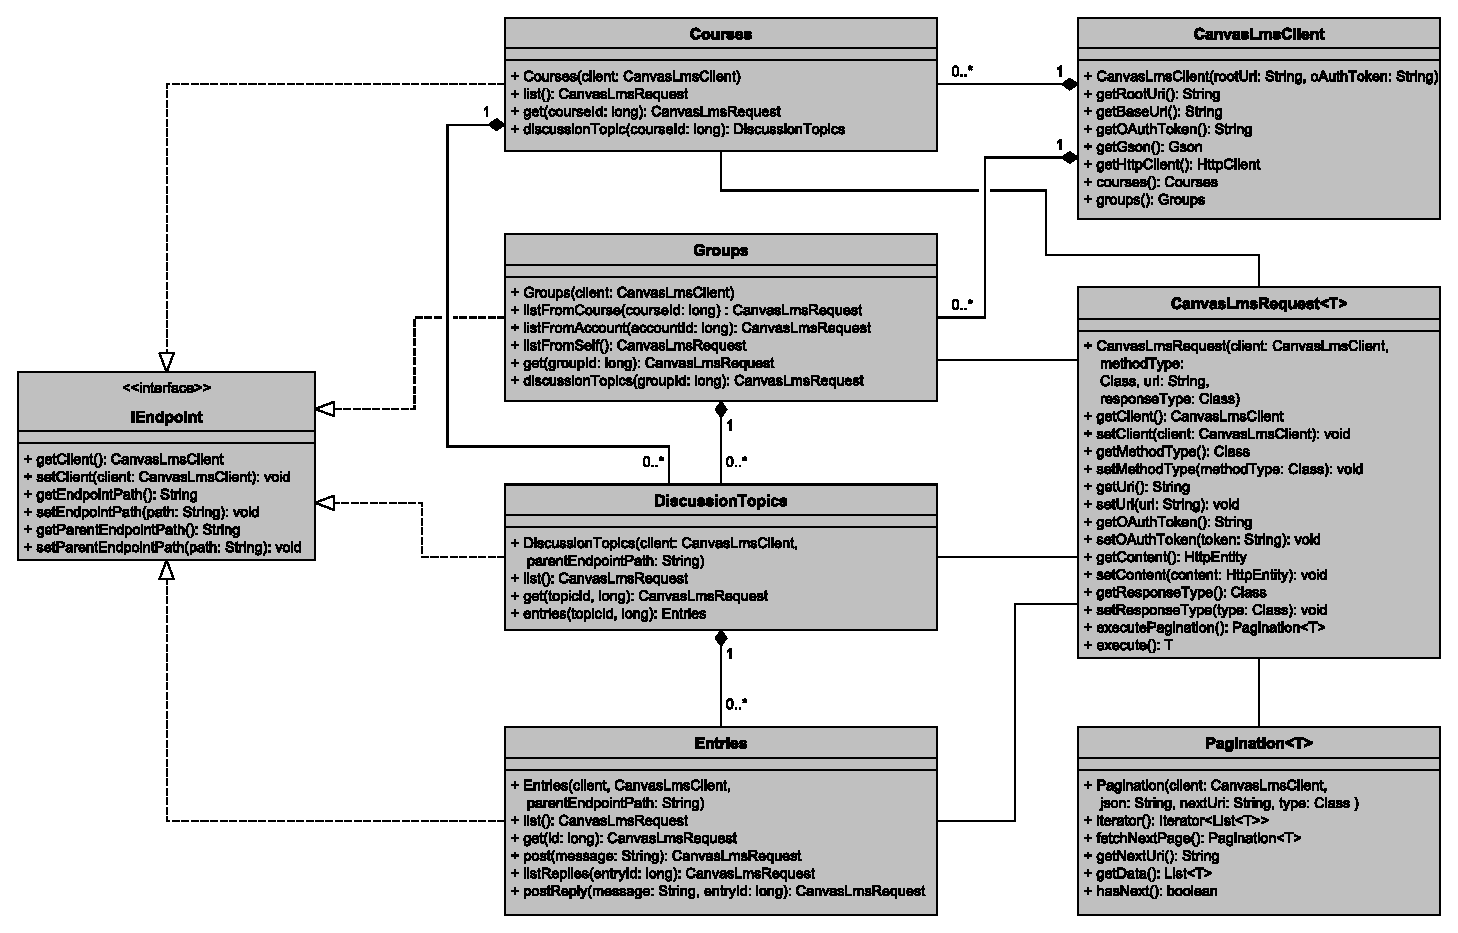
\includegraphics[
        width=\textwidth,
        keepaspectratio=true,]
    {assets/images/canvaslms4j_uml_classdiagramm}
    \caption{UML Klassendiagramm von CanvasLMS4J}
    \label{fig:canvaslms4j_uml_classdiagram}
\end{figure} 

Ausgangspunkt für CanvasLMS4J ist die Klasse \texttt{CanvasLmsClient} (siehe Abbildung \ref{fig:canvaslms4j_uml_classdiagram}). Über sie werden alle Endpunkte verwaltet die keinen Eltern-Endpunkt besitzen. Bei der Erzeugung eines Objektes dieser Klasse, werden ihr die URI zur verwendenden Canvas Instanz und der AccessToken des Benutzerkontos übergeben. Im aktuellen Stadium können von einem Client aus nur Endpunkte für Kurse oder Gruppe erstellt werden.

Endpunkte können dann über die Klasse \texttt{CanvasLmsRequest} REST-Anfragen an die Canvas API stellen. Hierzu verwendet CanvasLMS4J die \emph{HttpClient}\footnote{\url{http://hc.apache.org/httpclient-3.x/}} Bibliothek von Apache mit die einzelnen HTTP-Operationen ausgeführt werden. Um die im JSON-Format zurück gelieferten Antworten der Canvas API in Java verwenden zu können, wir auf die Funktionen der von Google entwickelten \emph{Gson}\footnote{\url{https://code.google.com/p/google-gson/}} Bibliothek zurück gegriffen. Sie erlaubt es Java Objekte in das JSON-Format zu konvertieren und genauso aus Daten in JSON ein Java Objekt zu machen. Dadurch verringert sich der Aufwand für das Verarbeiten der Daten von Canvas auf das Erstellen der entsprechenden Java Klassen. CanvasLmsRequest können mit zwei verschiedenen Methoden ausgeführt werden. Die erste \texttt{execute()} wird dazu verwendet, wenn die REST-Abfrage nur die Rückgabe eines Objektes zu Folge hat. Also zum Beispiel, wenn nur die Daten eines bestimmten Kurses abgefragt werden soll. Die zweite Methode ist \texttt{executePagination}. Diese Methode dient für Abfragen die eine in Seiten aufgeteilte Liste von Ergebnissen zurückliefert und gibt für eine einfache Handhabbarkeit ein Objekt der Klasse \texttt{Pagination} zurück. 

Die Klasse Pagination ist nach dem Iterator Muster aufgebaut und liefert vom kompletten Ergebnis bei jedem Iterationsschritt eine Seite zurück. Diese Seite enthält dann je eine Teilliste der angefragten Objekten. Ist eine Seite fertig ausgelesen, holt Pagination über eine vorgegeben REST Abfrage die nächste Seite. Dies geschieht solange bis keine Seiten mehr geladen werden können oder das Programm das Lesen abbricht.

\begin{lstlisting}[
    caption={CanvasLMS4J Beispielprogramm}\label{lst:canvaslms4j_beispiel},
    captionpos=t]
CanvasLmsClient client = new CanvasLmsClient(
                "https://canvas.instructure.com",
                "7~LUpV7B3lJY...");

Pagination<DiscussionTopic> discussionPages = client.courses()
    .discussionTopics( 798152 )
    .list()
    .executePagination();


for ( List<DiscussionTopic> discussions : discussionPages ) {
    for ( DiscussionTopic discussion : discussions ) {
        System.out.println( discussion );
    }
}

\end{lstlisting}

In Listing \ref{lst:canvaslms4j_beispiel} ist ein Beispiel für die Anwendung der CanvasLMS4J API zu sehen. In den ersten drei Zeilen wird eine neuer CanvasLmsClient für die Canvas Instanz auf \texttt{https://canvas.instructure.com} und einem AccessToken erstellt. Als nächstes soll für einen Kurs mit der ID \enquote{798152} alle Diskussionen aufgelistet werden. Mit dem Aufruf der Methode \texttt{courses()} des Clients wir der Endpunkt für die Kurse und von diesem aus der Endpunkt für die Diskussionen im Kurs \enquote{798152} über die Methode \texttt{.discussionTopics( 798152 )}. In der siebten Zeile wird die Art der Abfrage genauer festgelegt. Da eine Liste alle Diskussionen gesucht ist, wird die Methode \texttt{list()} aufgerufen die ein CanvasLmsRequest Objekt für die gewünschte Abfrage erstellt. Da die Antwort aus mehrere Objekten mit der Beschreibung der einzelnen Diskussionen besteht, wird die Anfrage in Zeile Acht mit der Methode \texttt{executePagination()} ausgeführt. Die einzelnen Seiten des Ergebnisses werden dann in der elften Zeile mit einer For-Schleife durchlaufen. Das nachladen der Seiten erfolgt dabei automatisch durch die Pagination Klasse. Jede Seite besteht nun aus einer Liste mit den Beschreibung der Diskussionen in einem \texttt{DiskussionTopic} Objekt, welche dann wieder in einer weiteren Schleife ausgegeben werden.

% subsubsection canvaslms4j (end)

\subsubsection{Canvas Mapping nach SIOC} % (fold)
\label{ssub:canvas_sioc_mapping}

\begin{table}[ht]
    \centering
    \caption{Format der URIs für Canvas}
    \begin{tabular}{l|p{11cm}}
        \textbf{URI Platzhalter} & URI-Format \\ 
        \hline
        \texttt{\{serviceUri\}} & 
        \texttt{\{rootUri\}/api/v1} \\

        \texttt{\{userAccountUri\}} & 
        \texttt{\{rootUri\}/about/\{userId\}} \\

        \texttt{\{siteUri\}} & 
        \texttt{\{rootUri\}} \\

        \texttt{\{forumUri\}} & 
        \texttt{\{rootUri\}/courses/\{courseId\}},
        \texttt{\{rootUri\}/groups/\{groupId\}} \\

        \texttt{\{threadUri\}} & 
        \texttt{\{forumUri\}/discussion\_topics/\{topicId\}} \\

        \texttt{\{postUri\}} & 
        \texttt{\{threadUri\}/entries/\{entryId\}},
        \texttt{\{threadUri\}\#discussion\_topic} \\
    \end{tabular}
    \label{tbl:canvas_uri_platzhalter}
\end{table}

% subsubsection canvas_sioc_mapping (end)

% subsection canvas_connector (end)

% section implementierung_einiger_connectoren (end)

\section{Evaluation} % (fold)
\label{sec:evaluation}

% section evaluation (end)

% chapter implementierung_und_evaluation (end)
		%!TEX root = ../thesis.tex

\chapter{Zusammenfassung und Ausblick} % (fold)
\label{cha:zusammenfassung_und_ausblick}

Im letzten Kapitel sollen noch einmal alle Ergebnisse diese Arbeit zusammengefasst und einen Ausblick auf weiterführende Themen gegeben werden. In der Einleitung wurde beschrieben, dass Diskussionen ein wichtiger Bestandteil des E-Learnings ist, aber diese oftmals auf verschiedene Plattformen verteilt stattfinden. Dadurch verpassen Personen, die nur auf einer dieser Plattformen präsent sind, vielleicht für sie wichtige Informationen auf einer anderen. Außerdem werden die selben Diskussionsthemen immer wieder an unterschiedlichen Orten an den unterschiedlichsten Orten doppelt und dreifach behandelt. Aus diesem Grund sollte ein System entwickelt werden das den Austausch von Diskussionen zwischen den unterschiedlichen Plattformen ermöglicht. 

In Kapitel \ref{cha:analyse} wurde analysiert, welche Schritte für eine solche Synchronisation nötig sind. Zuerst musste eine Zwischenformat gefunden werden in das die Daten der unterschiedlichen Plattformen konvertiert werden konnten, da dieser Weg effizienter ist, als die einzelnen Formate untereinander zu konvertieren. Also ein solches Zwischenformat bat sich die SIOC Ontologie in Verbindung mit FOAF wunderbar an. Ontologien bietet nicht nur einen guten Ansatz für die Integration von unterschiedlichen Datenformaten, mit RDF ist es sogar möglich dass Programme diese Daten verstehen und aus ihnen neues Wissen ableiten können. Um die Daten letztendlich in das Zwischenformat konvertieren und verarbeiten zu können, braucht es eine einheitliche Schnittstelle mit der dies umgesetzt werden kann. Zusätzlich wurde noch ein System gebraucht, dass die konvertierten Daten zwischen den Schnittstellen für die einzelnen Plattformen austauscht. Zu eignete sich der Austausch über Nachrichten am besten, da dadurch die einzelnen Schnittstellen zeitlich und räumlich entkoppelt werden konnten und nicht voneinander abhängig sind. Als Basis für dieses Nachrichtensystem wurde dann Apache Camel ausgewählt. Mit dieser Java-Bibliothek können die Routen, welche die Nachrichten nehmen, flexibel konfiguriert werden und sind so leicht erweiterbar. Privatsphäre spielt in der heutigen Zeit ebenfalls ein wichtige Rolle. Deswegen muss es Benutzern es ermöglicht werden das automatischen Lesen und/oder Schreiben für seine Beiträge zuzustimmen oder abzulehnen.

Das Kapitel \ref{cha:eigener_ansatz_social_online_community_connectors_socc_} widmet sich der Beschreibung des Systems, welches alle notwendigen Schritte und Anforderungen aus Kapiel \ref{cha:analyse} erfüllt. Dieses System, dass SOCC getauft wurde, besteht aus Connectoren die für das Lesen, Konvertieren und Schreiben für die Plattformen verantwortlich sind und einer Komponente die diese Connectoren in Apache Camel integriert. 


\section{Ausblick} % (fold)
\label{sec:ausblick}

% section ausblick (end)

% chapter abschlussbetrachtung (end)
		\cleardoublepage

	\appendix
	    %!TEX root = ../thesis.tex

\chapter{Anhang} % (fold)
\label{cha:anhang}

\section{SOCC Connector Config Ontologie} % (fold)
\label{sec:anhang_socc_connector_config_ontologie}

\lstinputlisting[language=XML,caption={}]{assets/listings/socc-config.owl}

% section socc_connector_config_ontologie (end)

\section{SIOC Services Authentication Module} % (fold)
\label{sec:anhang_sioc_services_authentication_module}

\lstinputlisting[language=XML,caption={}]{assets/listings/sioc-service-auth.owl}

% section sioc_services_authentication_module (end)

\section{Proof of Concept: Konfigurationsdaten} % (fold)
\label{sec:anhang_proof_of_concept_konfigurationsdaten}

\lstinputlisting[language={},caption={}]{assets/listings/poc_config_model.ttl}

% section proof_of_concept_konfigurationsdaten (end)

% chapter anhang (end)
		%!TEX root = ../thesis.tex

%\addcontentsline{toc}{chapter}{Literaturverzeichnis}
\bibliographystyle{abbrv}
\bibliography{bibliography/literature,bibliography/online}

\end{document}

% Einleitung
%     (Motivation)
%     (Anforderungen)
%     (Kapitelübersicht)

% Grundlagen und verwandte Arbeiten
%     Datenintegration 
%         (Zusammenführen von Daten aus verschiedenen Quellen)
%         RDF
%         SIOC
%     Verwandte Arbeiten/Projekte
%         Reclaim
%         Glue!-PS

% Analyse
%     (Was fehlt bei verwandten Arbeiten)
%     Einheitliche Schnittstelle
%     MessagePassing
%         JMS vs Apache Camel  vs JMS + Apache Camel

% Eigener Ansatz
%     Verwendung von SIOC (RDF2Go...)
%     Connectoren Konzept
%         Moodle
%         Canvas LMS
%         Facebook
%         Youtube
%         Google+

% Evaluation
%     Auswertung was alles erreicht wurde

% Fazit und Ausblick